\documentclass{scrreprt}
\usepackage{listings}
\usepackage{underscore}
\usepackage[margin=2cm]{geometry}
\usepackage{graphicx}
\usepackage[bookmarks=true]{hyperref}
\usepackage[utf8]{inputenc}
\usepackage[english]{babel}
\usepackage[super]{nth}
\usepackage{placeins}
\usepackage[table,xcdraw]{xcolor}
\usepackage{array}
\usepackage{float}
\usepackage{xcolor,listings}
\usepackage{textcomp}
\usepackage{color}

\usepackage{etoolbox}
\makeatletter
\patchcmd{\scr@startchapter}{\if@openright\cleardoublepage\else\clearpage\fi}{}{}{}
\makeatother


\setlength{\parindent}{0em}
% \setlength{\parskip}{1.0em}

\definecolor{mygreen}{rgb}{0,0.6,0}
\definecolor{mygray}{rgb}{0.5,0.5,0.5}
\definecolor{mymauve}{rgb}{0.58,0,0.82}
\definecolor{darkgray}{rgb}{.4,.4,.4}
\definecolor{purple}{rgb}{0.65, 0.12, 0.82}

\lstset{ %
backgroundcolor=\color{white}, % choose the background color; you must add \usepackage{color} or \usepackage{xcolor}
basicstyle=\footnotesize, % the size of the fonts that are used for the code
breakatwhitespace=false, % sets if automatic breaks should only happen at whitespace
breaklines=true, % sets automatic line breaking
captionpos=b, % sets the caption-position to bottom
commentstyle=\color{mygreen}, % comment style
deletekeywords={...}, % if you want to delete keywords from the given language
escapeinside={\%*}{*)}, % if you want to add LaTeX within your code
extendedchars=true, % lets you use non-ASCII characters; for 8-bits encodings only, does not work with UTF-8
frame=single, % adds a frame around the code
keepspaces=true, % keeps spaces in text, useful for keeping indentation of code (possibly needs columns=flexible)
keywordstyle=\color{blue}, % keyword style
language=Octave, % the language of the code
morekeywords={*,...}, % if you want to add more keywords to the set
numbers=left, % where to put the line-numbers; possible values are (none, left, right)
numbersep=5pt, % how far the line-numbers are from the code
numberstyle=\tiny\color{mygray}, % the style that is used for the line-numbers
rulecolor=\color{black}, % if not set, the frame-color may be changed on line-breaks within not-black text (e.g. comments (green here))
showspaces=false, % show spaces everywhere adding particular underscores; it overrides 'showstringspaces'
showstringspaces=false, % underline spaces within strings only
showtabs=false, % show tabs within strings adding particular underscores
stepnumber=1, % the step between two line-numbers. If it's 1, each line will be numbered
stringstyle=\color{mymauve}, % string literal style
tabsize=2, % sets default tabsize to 2 spaces
title=\lstname % show the filename of files included with \lstinputlisting; also try caption instead of title
}

\lstdefinelanguage{JavaScript}{
keywords={typeof, new, true, false, catch, function, return, null, catch, switch, var, if, in, while, do, else, case, break},
keywordstyle=\color{blue}\bfseries,
ndkeywords={class, export, boolean, throw, implements, import, this},
ndkeywordstyle=\color{darkgray}\bfseries,
identifierstyle=\color{black},
sensitive=false,
comment=[l]{//},
morecomment=[s]{/*}{*/},
commentstyle=\color{purple}\ttfamily,
stringstyle=\color{red}\ttfamily,
morestring=[b]',
morestring=[b]"
}
\lstset{
language=JavaScript,
extendedchars=true,
basicstyle=\footnotesize\ttfamily,
showstringspaces=false,
showspaces=false,
numbers=left,
numberstyle=\footnotesize,
numbersep=9pt,
tabsize=2,
breaklines=true,
showtabs=false,
captionpos=b
}

\addtokomafont{disposition}{\rmfamily}
%}
\usepackage{hyperref}

\pagenumbering{gobble}

\title{F21DV Coursework Part 1 Report}
\author{Jonathan Song Yang, Lee}
\date{H00255553}

\begin{document}

\maketitle

\newpage
\tableofcontents

\pagenumbering{arabic}

\newpage
\chapter{Introduction}
The entirety of the F21DV four-part coursework is done in a way where it resembels
a full static or a \verb|node.js| server-side web application. The goal of this
series of coursework is to demonstrate the understanding of \verb|d3.js|.\\
\par Github Repo: \href{https://github.com/jonleesy/F21DV-Coursework}{https://github.com/jonleesy/F21DV-Coursework}\\
Github Pages: \href{https://jonleesy.github.io/F21DV-Coursework/public}{https://jonleesy.github.io/F21DV-Coursework/public}

\section{General Setup}
\begin{figure}[!ht]
    \centering
    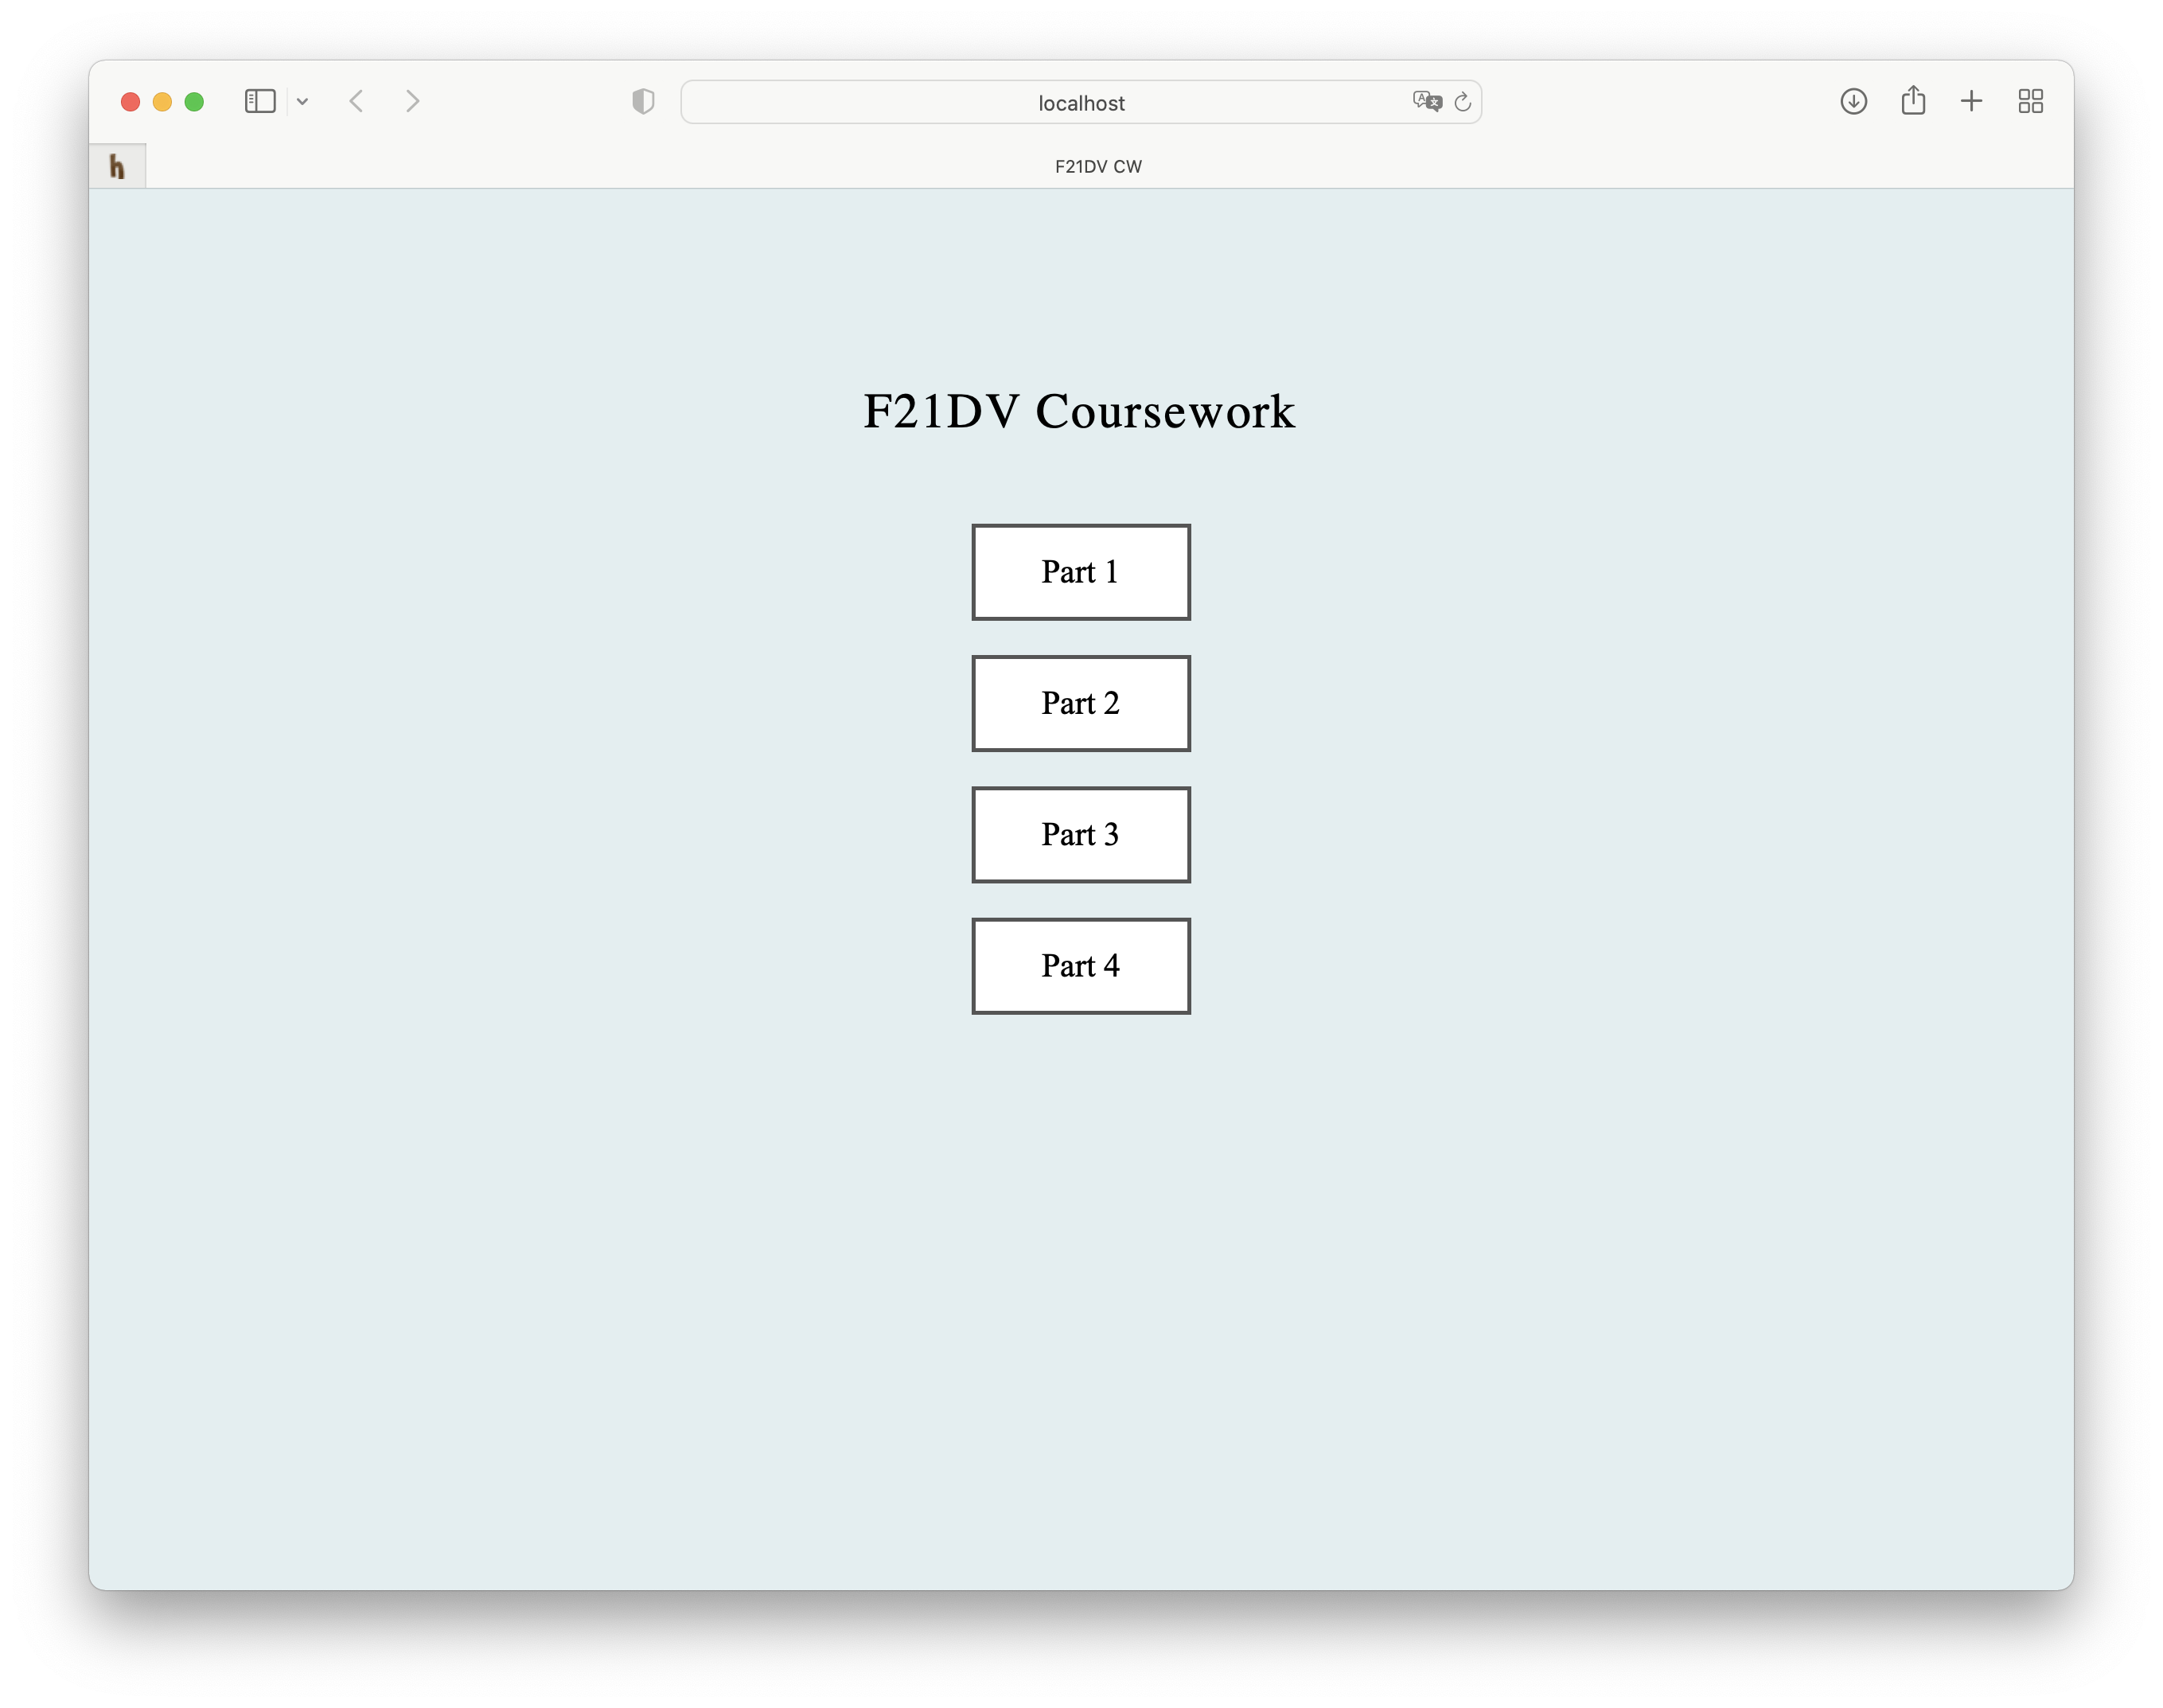
\includegraphics[width = 10cm]{images/main.png}
    \label{fig:main}
    \caption{Main Index Page}
\end{figure}
\FloatBarrier
The main index page of the web application would show buttons to access parts 1 to
4, as shown in figure \ref{fig:main}, and for the case of Lab 1, upon clicking on
the Part 1 button, a series of urls linking to different exercises would be shown,
as seen in figure \ref{fig:part1} below.
\begin{figure}[!ht]
    \centering
    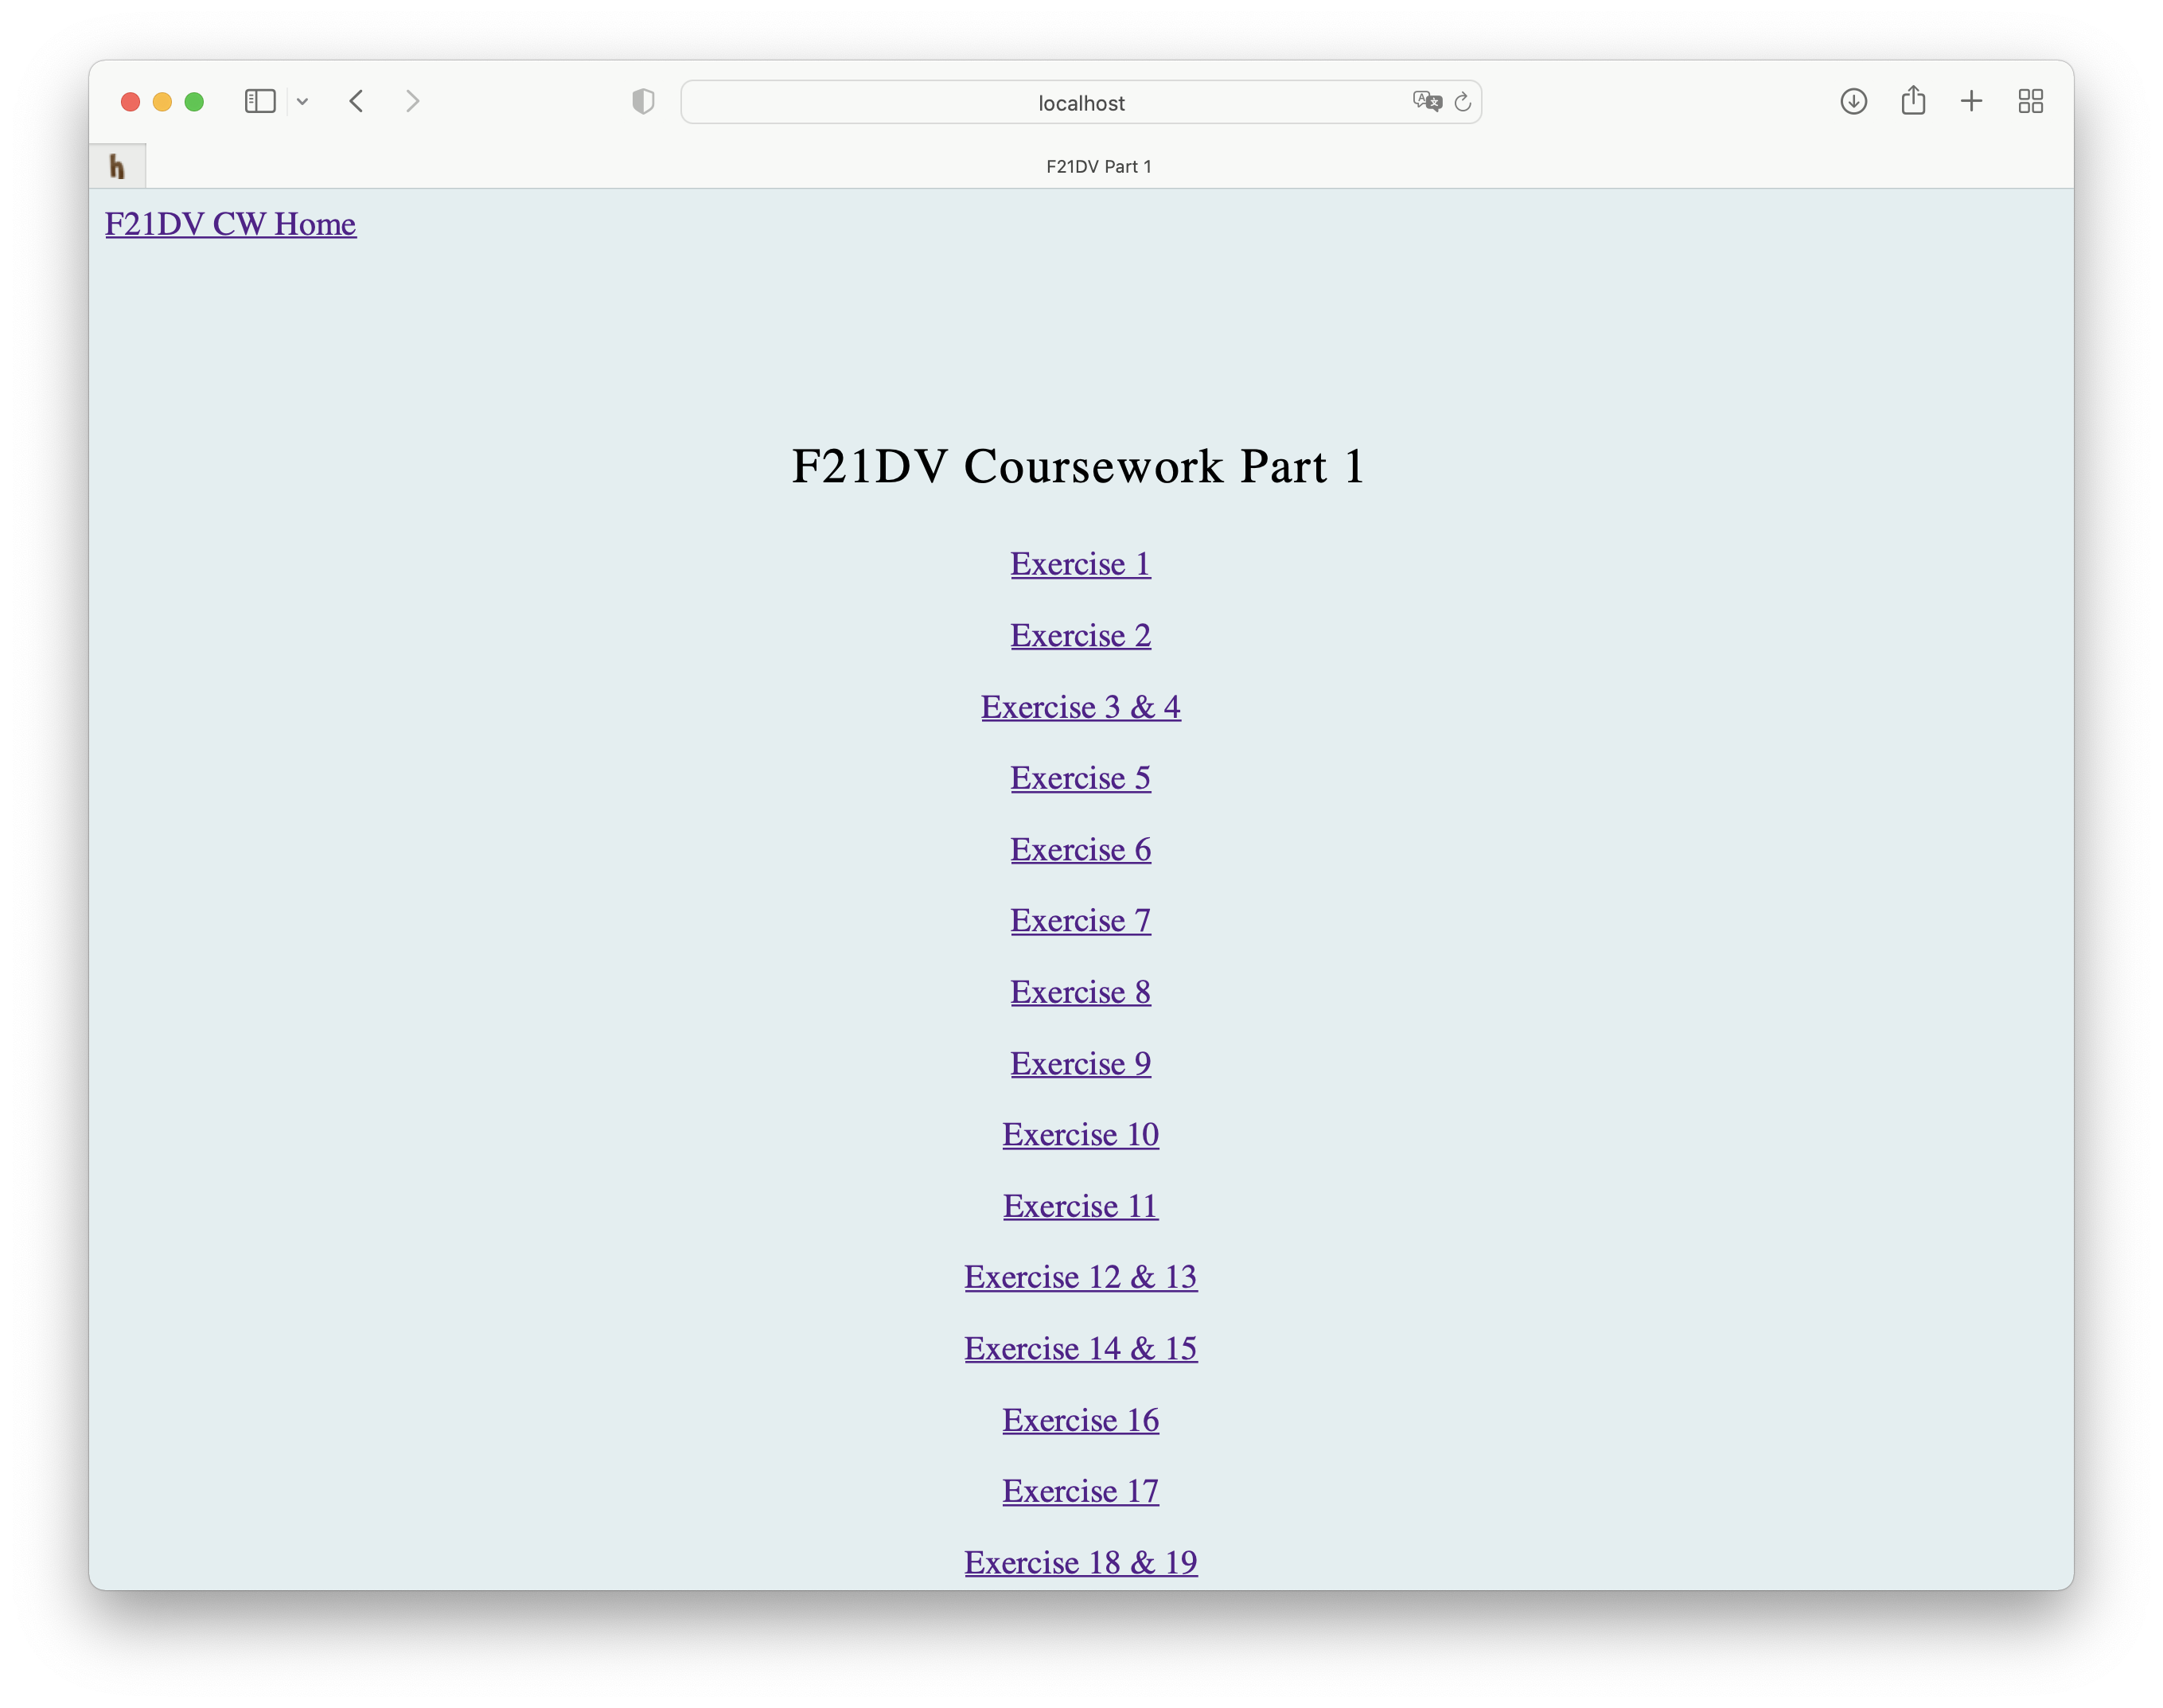
\includegraphics[width = 7cm]{images/part1_1.png}
    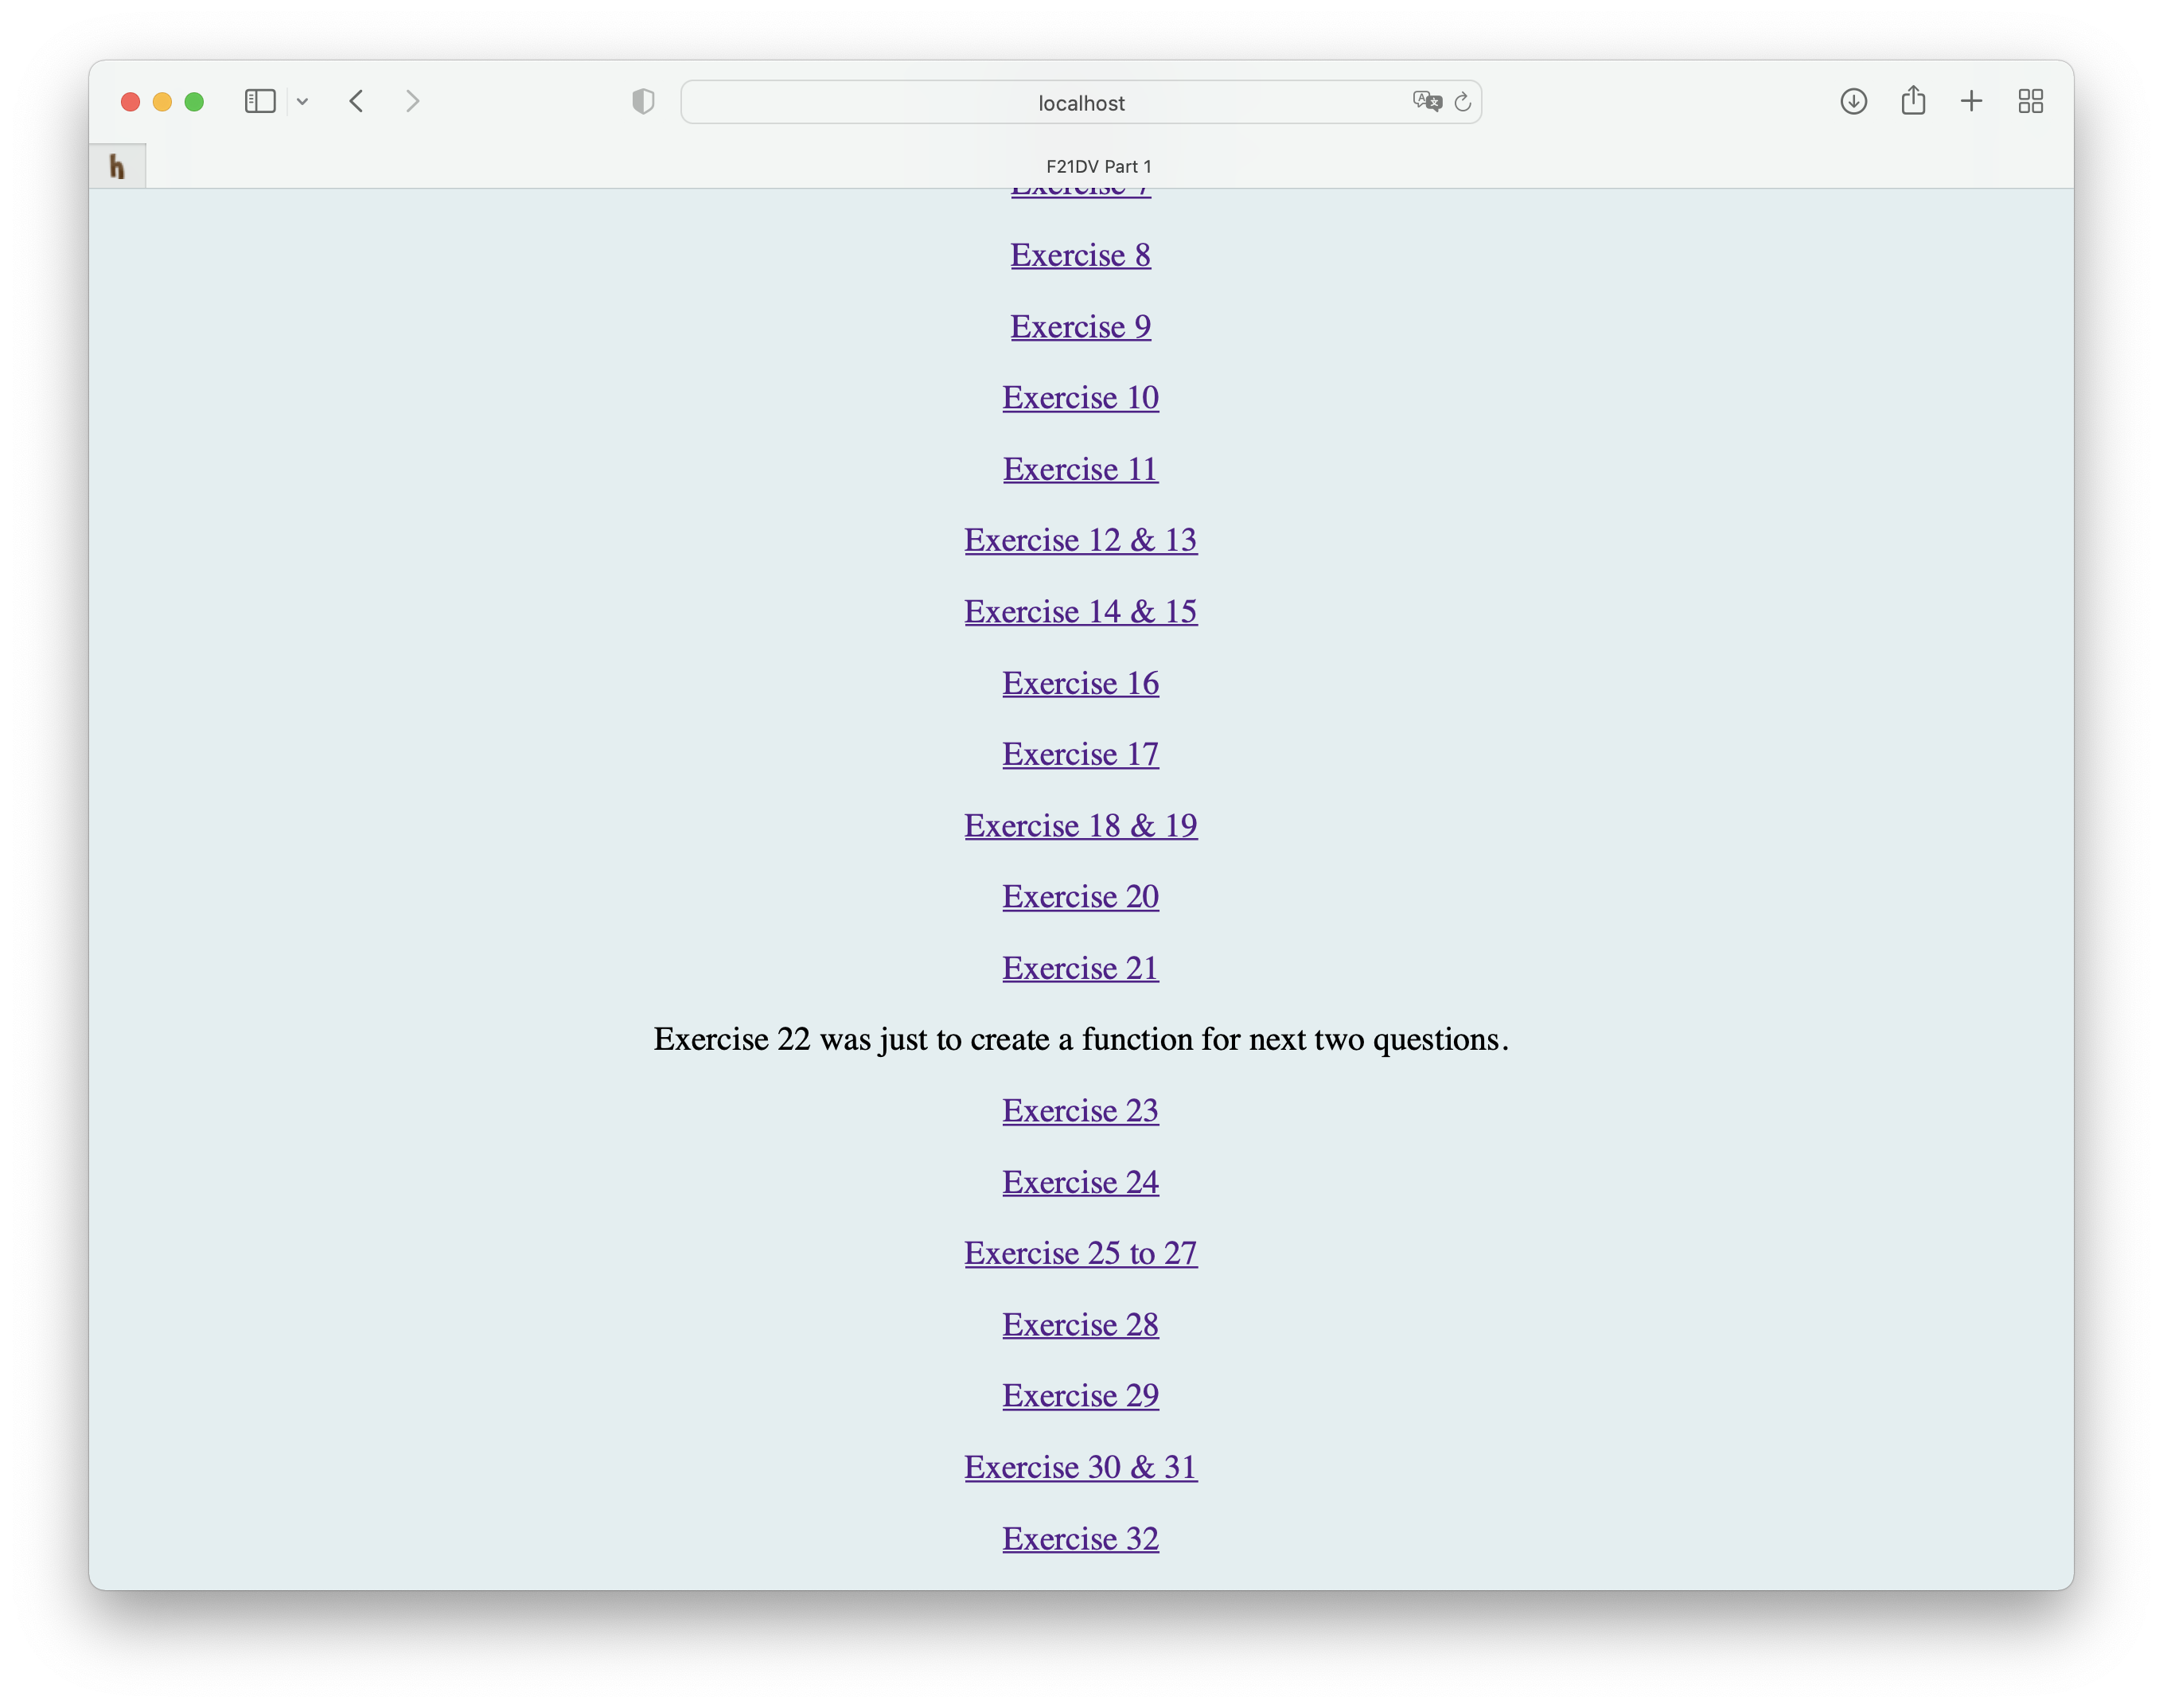
\includegraphics[width = 7cm]{images/part1_2.png}
    \label{fig:part1}
    \caption{Main Index Page}
\end{figure}
\FloatBarrier
To demonstrate the understanding of \verb|d3.js|, this series of URLs were created
systematically using \verb|d3.js|, as shown in listing \ref{lst:urlSystematic} abstact
below. 

\begin{lstlisting}[language=JavaScript,
                    caption={Systematic URL Creation},
                    captionpos=b,
                    label={lst:urlSystematic}]
    // Array of numbers [0, 1, 2, ..., 32] defining number of exercises
    const data = Array.from(Array(33).keys());

    // Creating links to 32 Exercises Systematically.
    d3.select('body').selectAll('p')
        .data(data)
        .enter()
            // Append a <p> for each exercise and add an <a> for each <p>
            .append('p').style('text-align', 'center')
                .attr('class', d => 'task' + d)
                .append('a')
                    .attr('href', d => 'task' + d +'.html')
                    .html(d => 'Exercise ' + d);
\end{lstlisting}

As the lab exercise would involve certain combinable exercises, such as exercises 30
and 31, I have also created a generalised function to help \textbf{combine} and
\textbf{delete} certain exercises.\\

\begin{lstlisting}[language=JavaScript,
    caption={Systematic URL Removal},
    captionpos=b,
    label={lst:taskSystematic}]
    /**
    * General Merge Function. If its just 2 consecutive exercise, ignore 3rd and 4th parameter. 
    * However, if merge is for a range of exercises, spanning more than 2, only enter the 
    * first and last exercise number.
    * @param {*} first first exercise to merge
    * @param {*} second second exercise to merge. Last exercise if there are more than 2 exercises.
    * @param {*} cond1 used to change exercise <number> to Exercise <number> to <number>
    * @param {*} cond2 used to rename html file to task<first>n<second>.html
    */
   function mergeTask(first, second, cond1 = ' \& ', cond2 = 'n') {
       d3.select('.task' + second).remove();
       d3.select('.task' + first + ' a').html('Exercise ' + first + cond1 + second)
                                           .attr('href', d => 'task' + first + cond2 + second + '.html');
   }
\end{lstlisting}
Listing \ref{lst:taskSystematic} shows a function that renames the href of combined exercises,
and removes and rename a pre-existing href. For example, we have initially Exercises 30 and 31.
The function first removes the exercise 31's \verb|<p>|, and then renames the original html href file
from \verb|task30.html| to \verb|task30n31.html|.\\

\begin{lstlisting}[language=JavaScript,
    caption={Systematic <a>-text Replacement},
    captionpos=b,
    label={lst:divReplaceSystematic}]
    // Remove task function
    function removeTask(task, message) {
        d3.select(`.task${task} a`).remove();
        d3.select(`.task${task}`).append('p')
                                .text(message);
    }
\end{lstlisting}
Listing \ref{lst:divReplaceSystematic} shows a generalised function that replaces the exercises URL
with a message string. For example, in exercise 22, we were asked to create a generalised SVG and
lines function. This function will now remove the \verb|href| from the \verb|<p>| element, and replace
it with a message string.


\newpage
\section{Individual Exercise HTMLs Setup}
Within each exercise's own HTML \verb|body|, they all inherit a generic CSS setting for a div called
\verb|.answerCenter| which acts as the center element for the presentation of answers for each
exercise. There is also a generic button cssd style called \verb|.buttonOri| and \verb|.button| that
handles the CSS transition of all the buttons. \\
\par For each exercise, I have also used a generalised function in \verb|functions.js| to create the
\verb|<div>|s and buttons so that the styles remain consistent across all exercises.\\
\begin{lstlisting}[language=JavaScript,
    caption={Systematic div and button creation},
    captionpos=b,
    label={lst:functionsjs}]
    /**
    * Create div's for each question systematically.
    * @param {*} exerciseNumber Task number.
    */
   export function createDiv(exerciseNumber) {
       d3.select('body')
           .append('div')
               .attr('class', 'container')
               .append('div')
                   .attr('class', 'answerCenter')
                   .append('p')
                       .append('strong')
                           .text('Exercise ' + exerciseNumber + ':')
   }
   
   /**
    * Creates a button to execute action for each task.
    * @param {*} exerciseNumber 
    */
   export function createButton(exerciseNumber) {
       d3.select('body')
           .append('div').attr('class', 'container')
               .append('div').attr('class', 'center')
                   .append('button')
                       .attr('class', 'buttonori')
                       .text('Click for Task ' + exerciseNumber)
   }
\end{lstlisting}
Listing \ref{lst:functionsjs} shows the systematic approach used to create the answer container, 
as well as buttons to execute exercises actions. However, not all exercise would use the button,
since not all exercise is in need of an action.

\newpage
\chapter{Exercises}
\section{Exercise 1}
\begin{figure}[!ht]
    \centering
    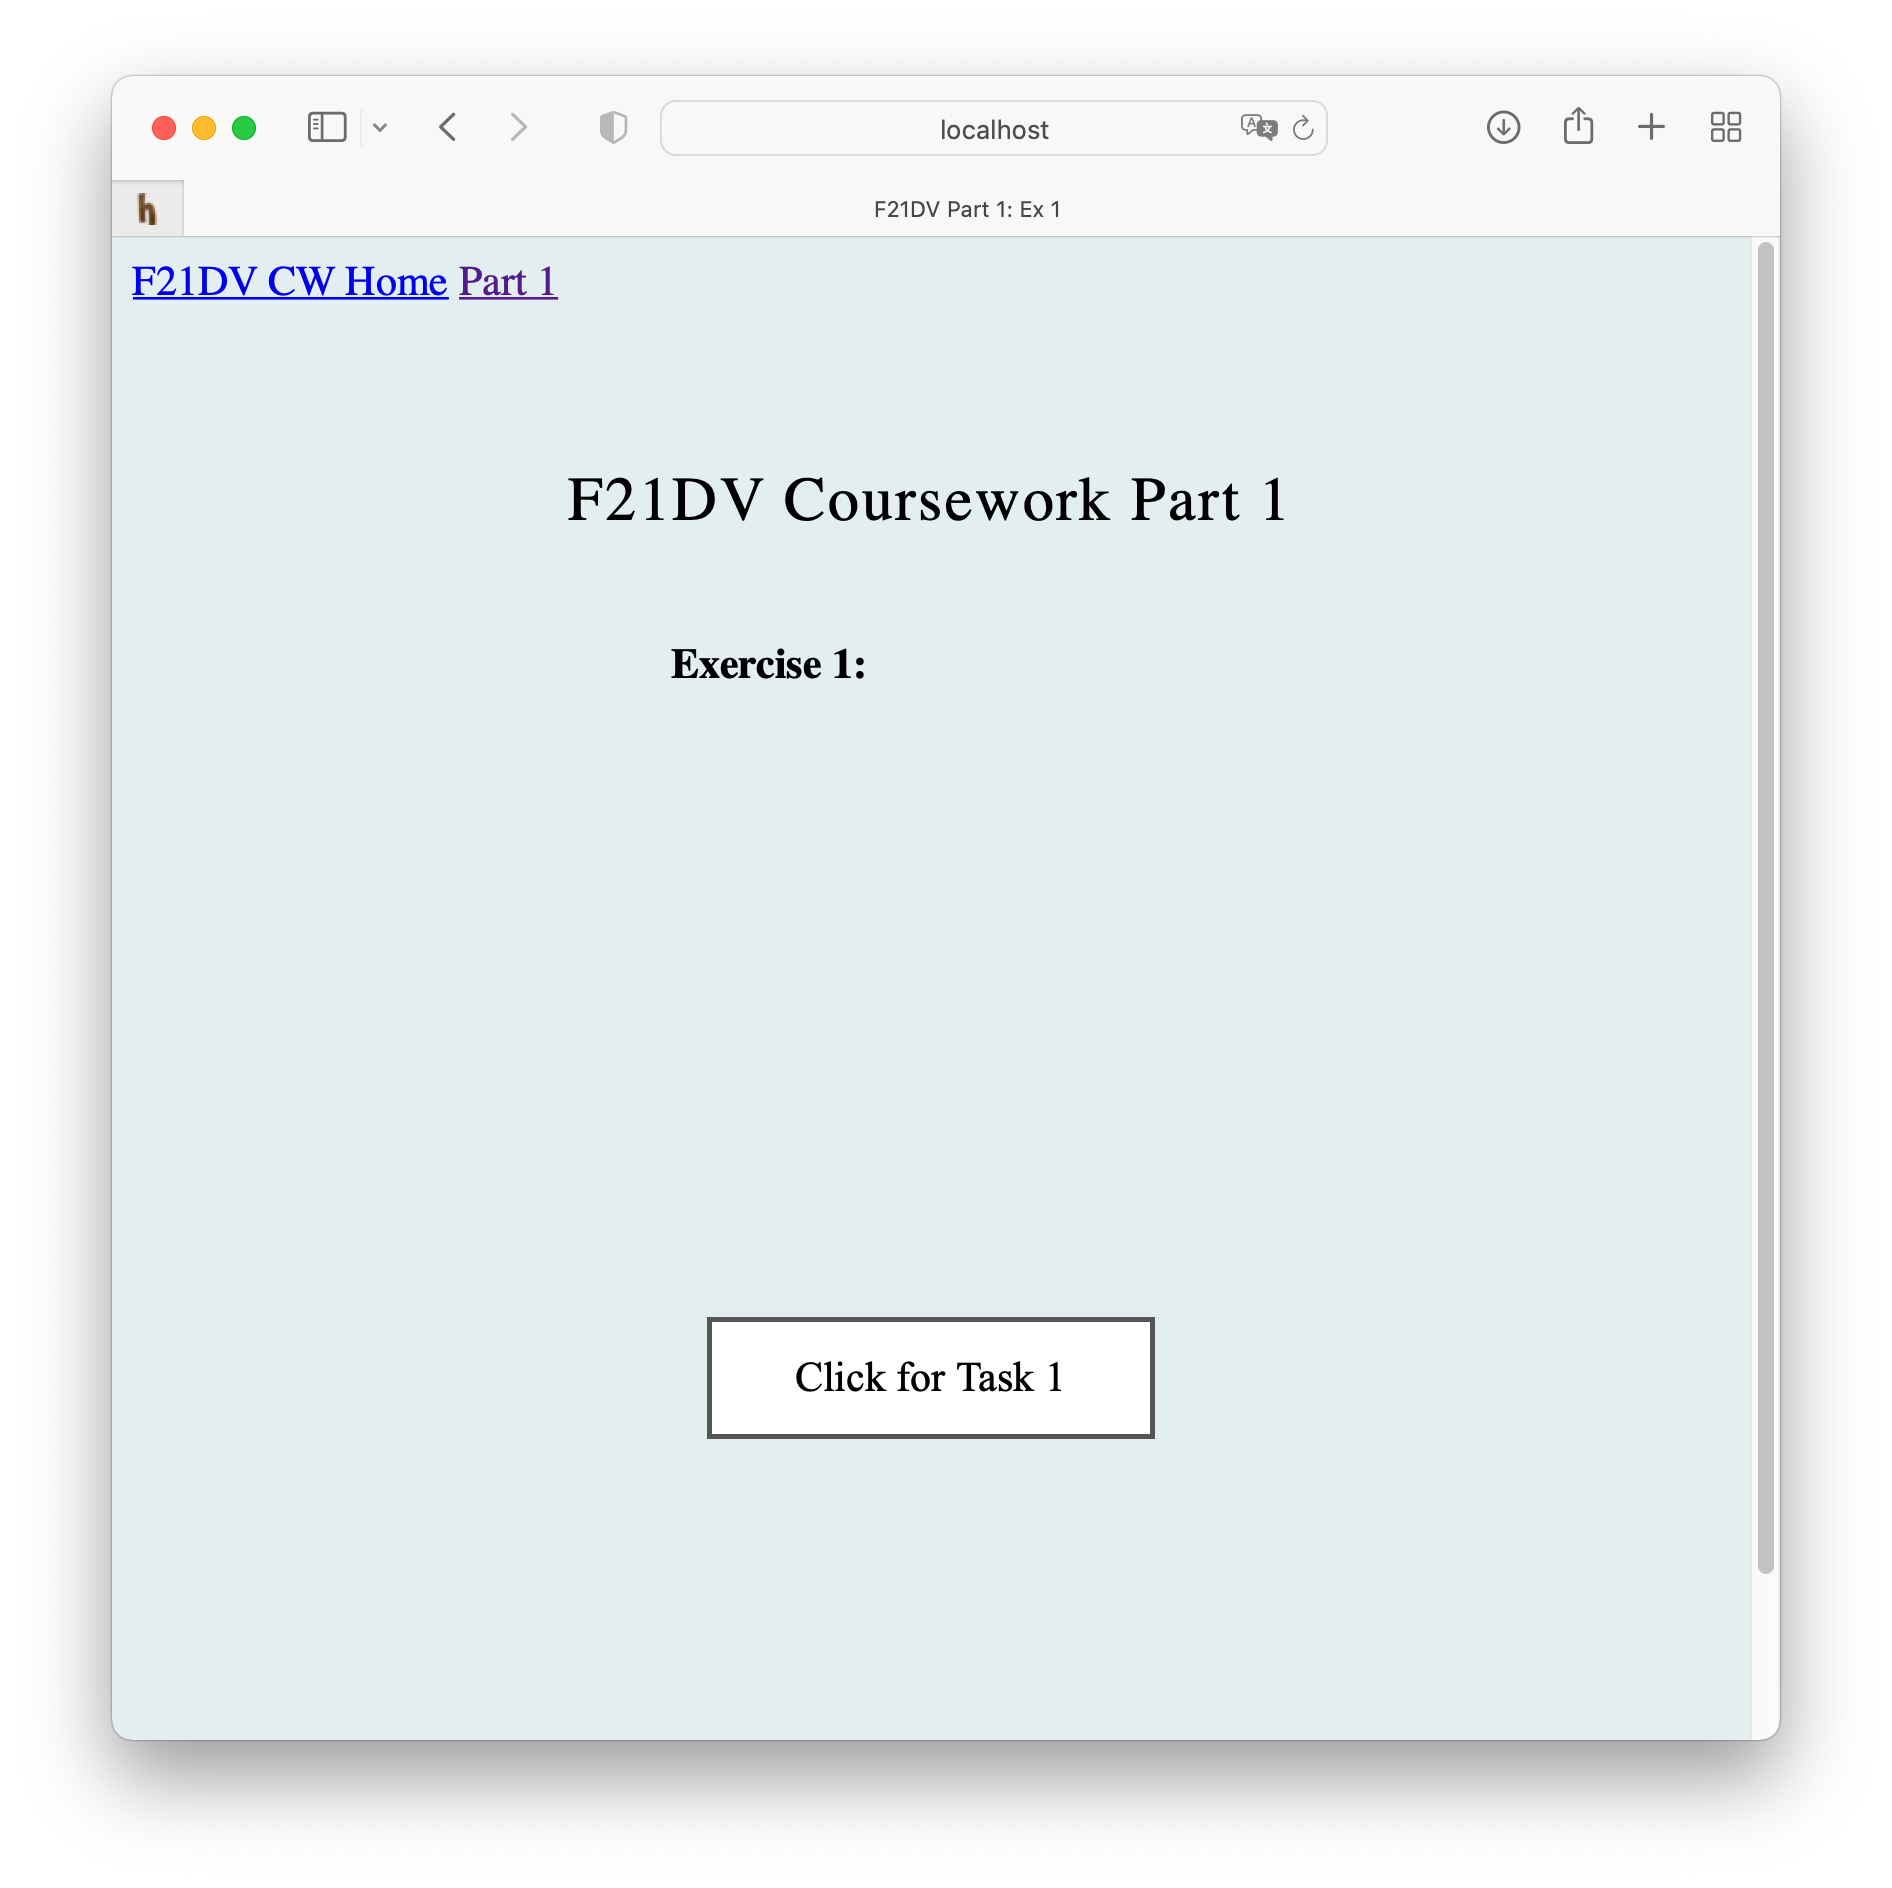
\includegraphics[width = 7.5cm]{images/ex1_1.png}
    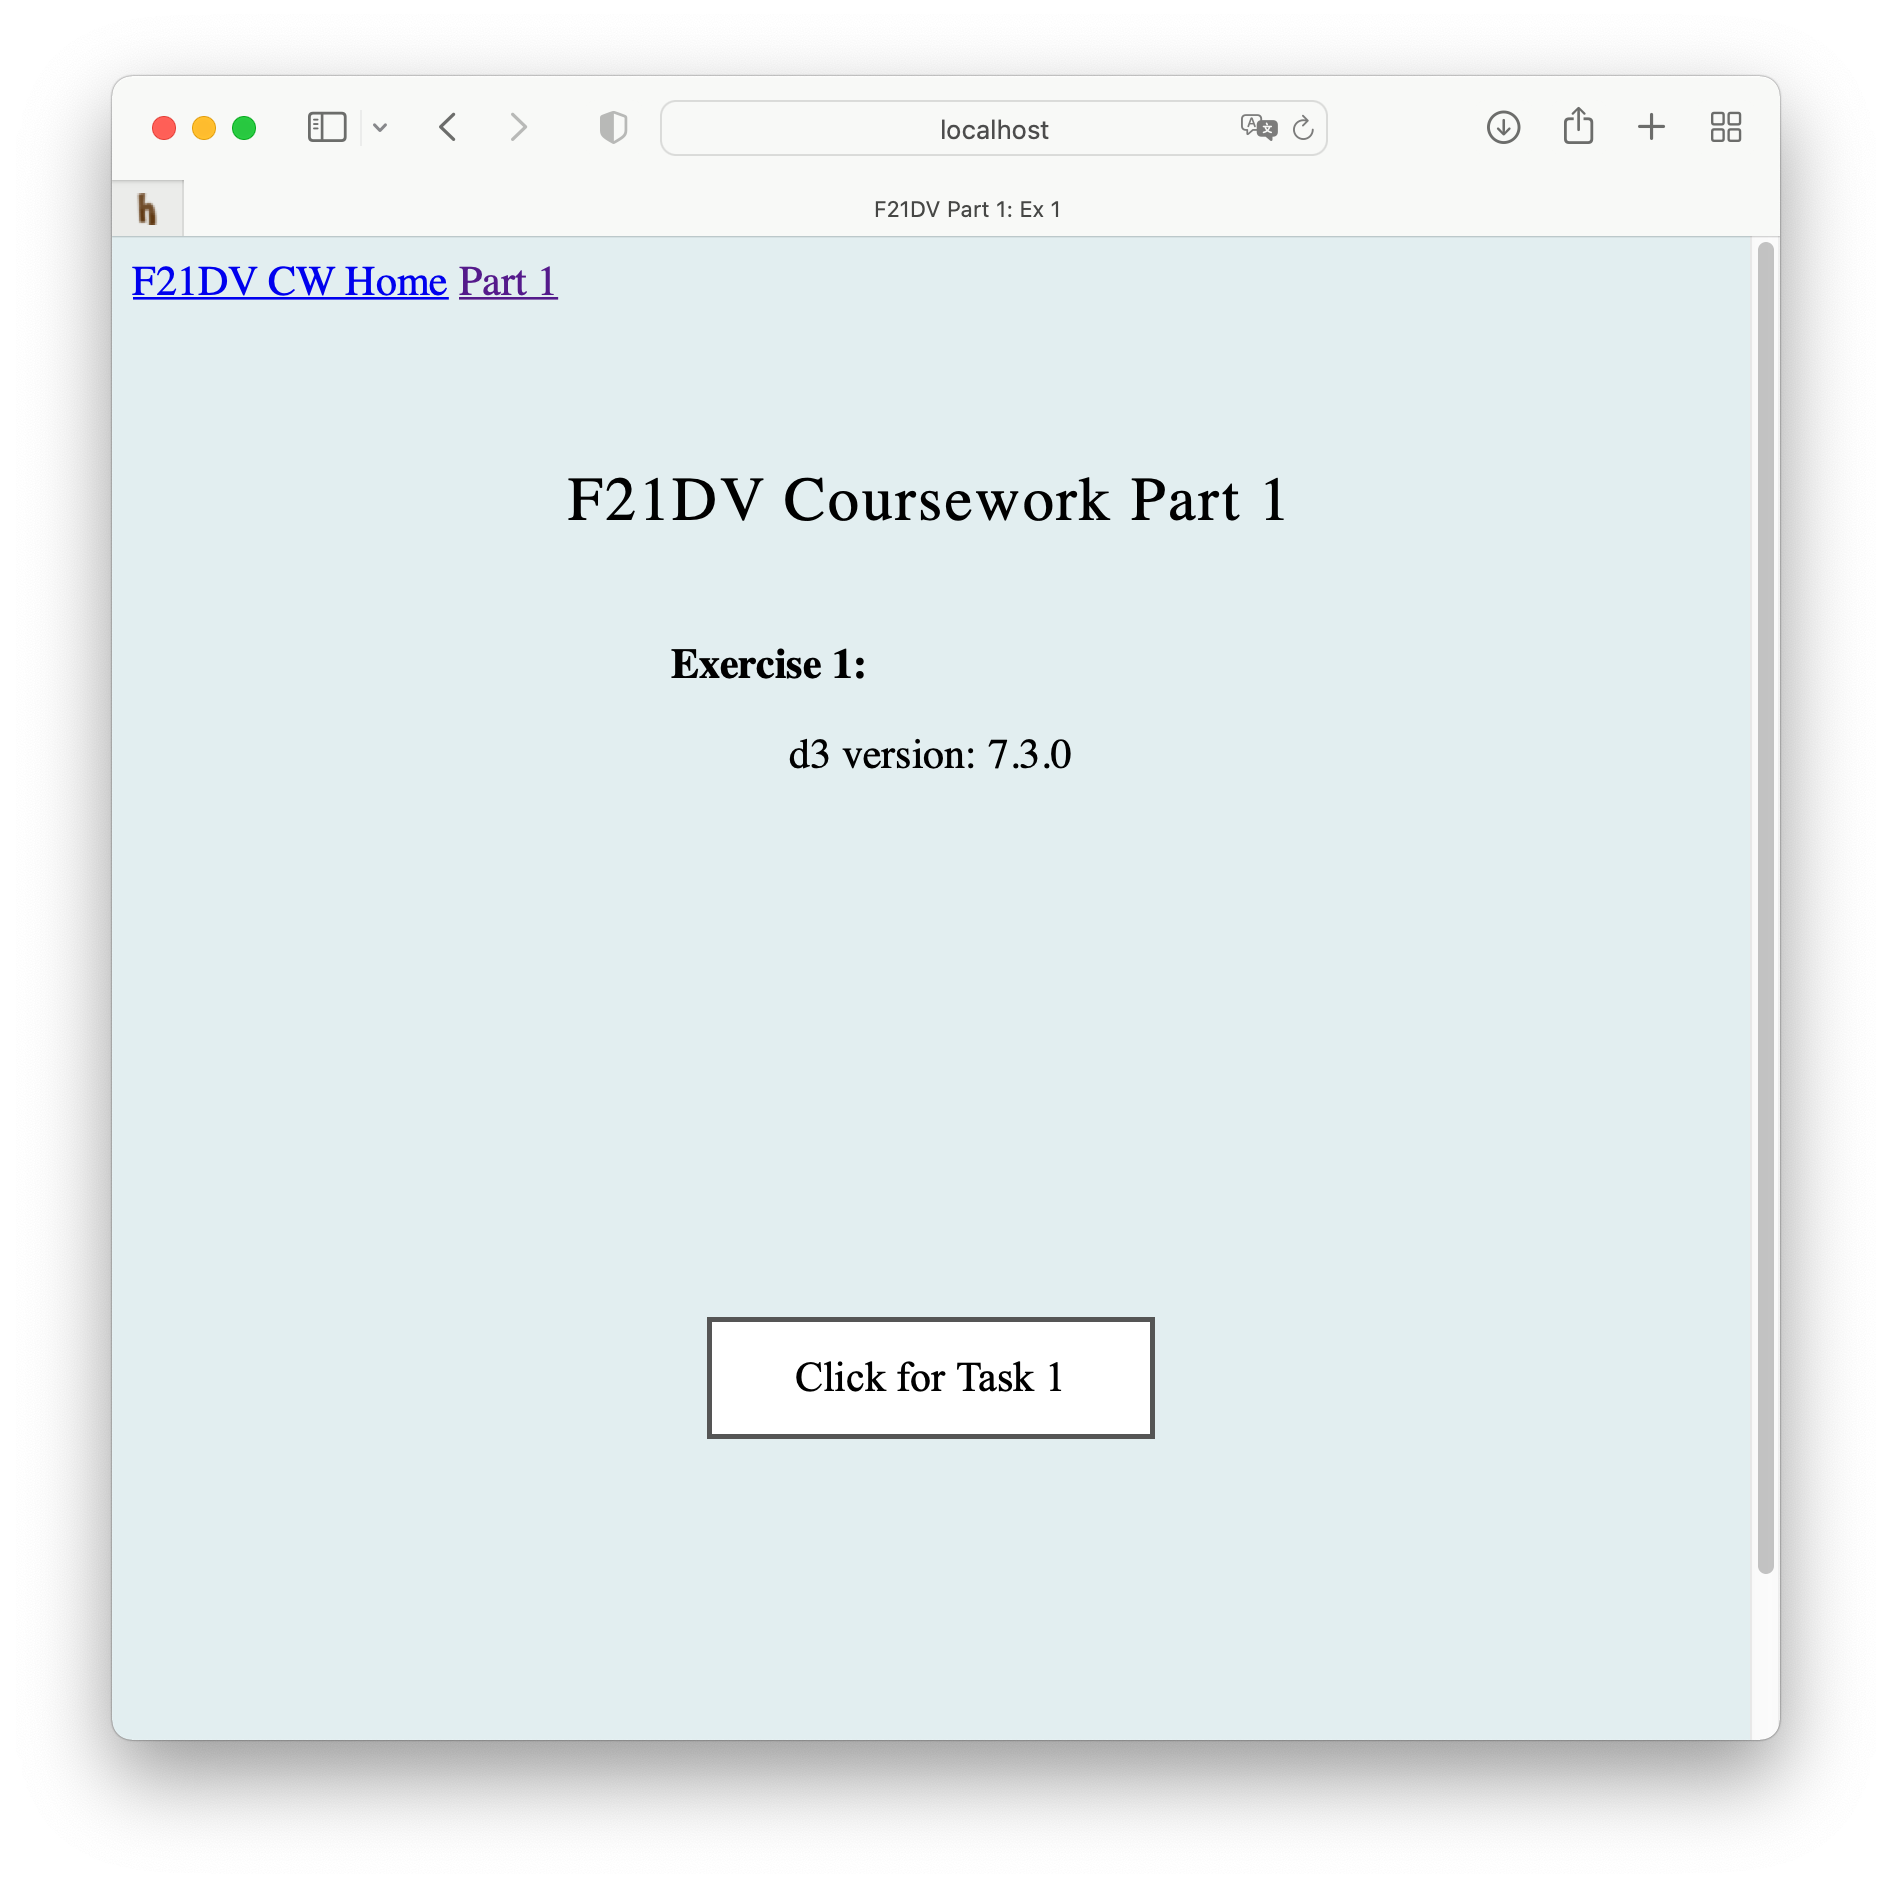
\includegraphics[width = 7.5cm]{images/ex1_2.png}
    \label{fig:ex1}
    \caption{Exercise 1}
\end{figure}
\FloatBarrier
Figure \ref{fig:ex1} shows the outcome after clicking on the action button. The answer container
space would print the d3 version number upon clicking the task button.
\lstinputlisting[language=JavaScript]{../../public/js/part1/task1.js}
Upon clicking the button, using d3, the button action replaces the empty \verb|<p>| with "d3
version: 7.3.0". For the remaining exercises, the button action would do a similar thing as well.
It would select the desired object for modification, and through a button on-click event listener,
modify the selected object.

\newpage
\section{Exercise 2}
\begin{figure}[!ht]
    \centering
    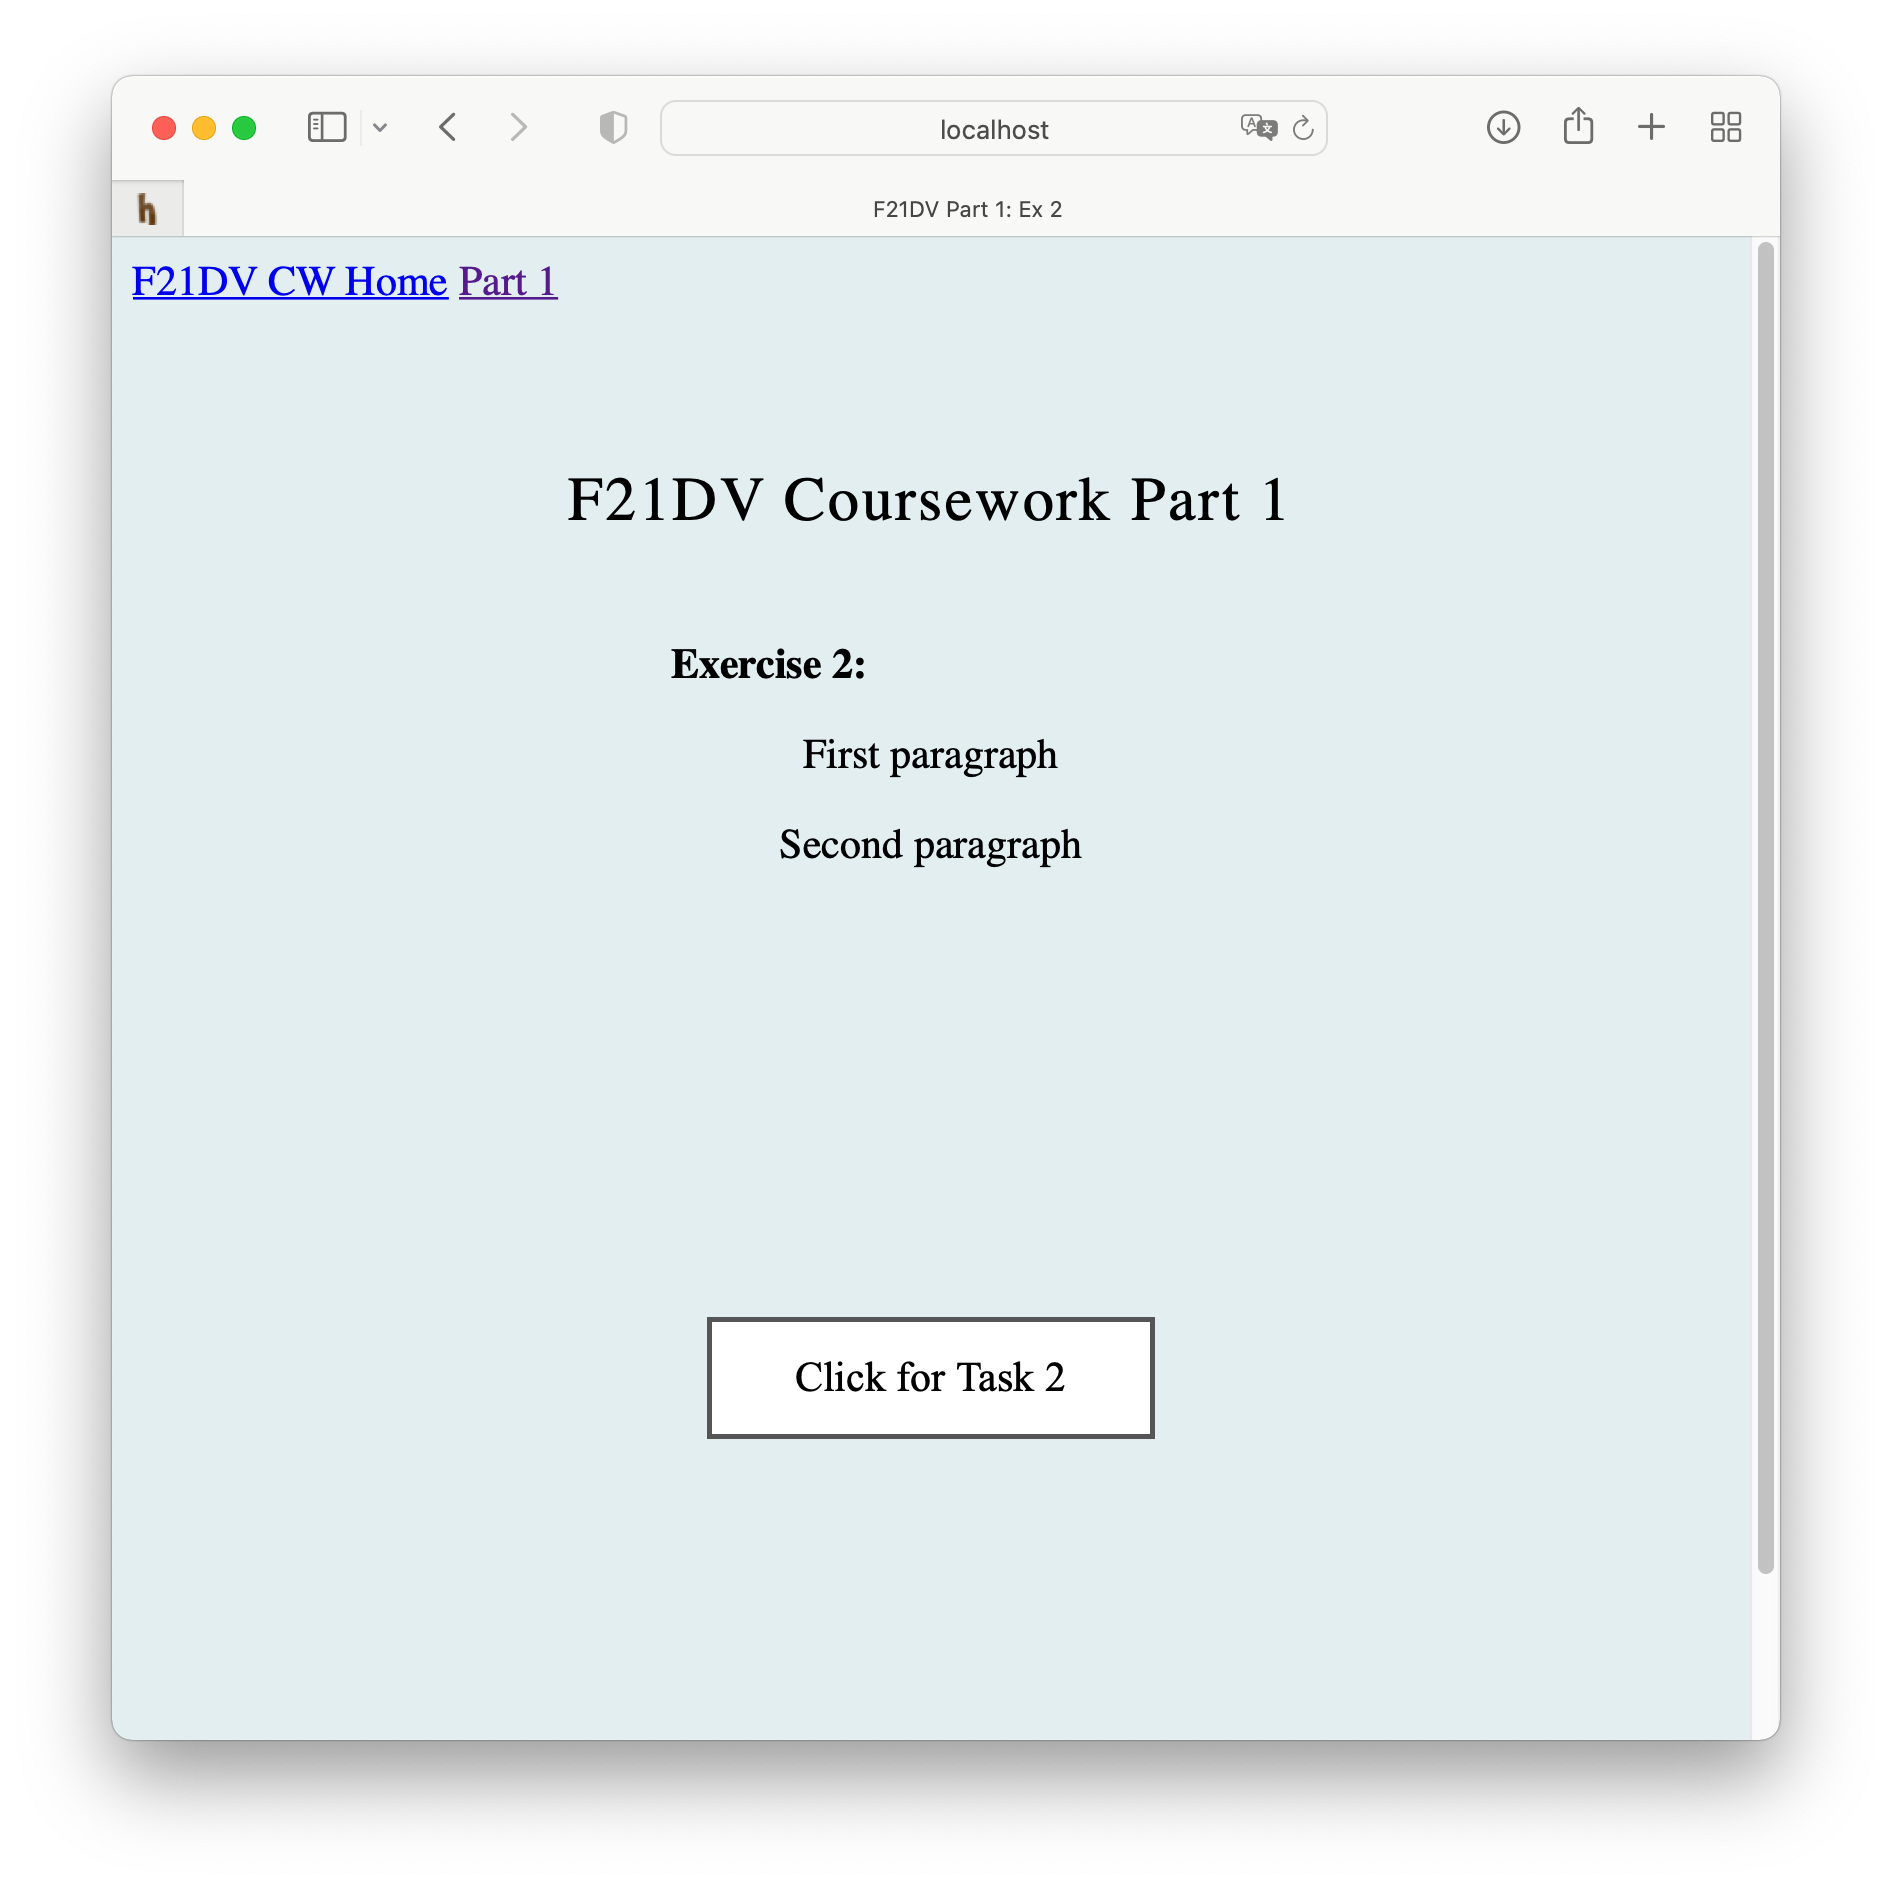
\includegraphics[width = 8cm]{images/ex2_1.png}
    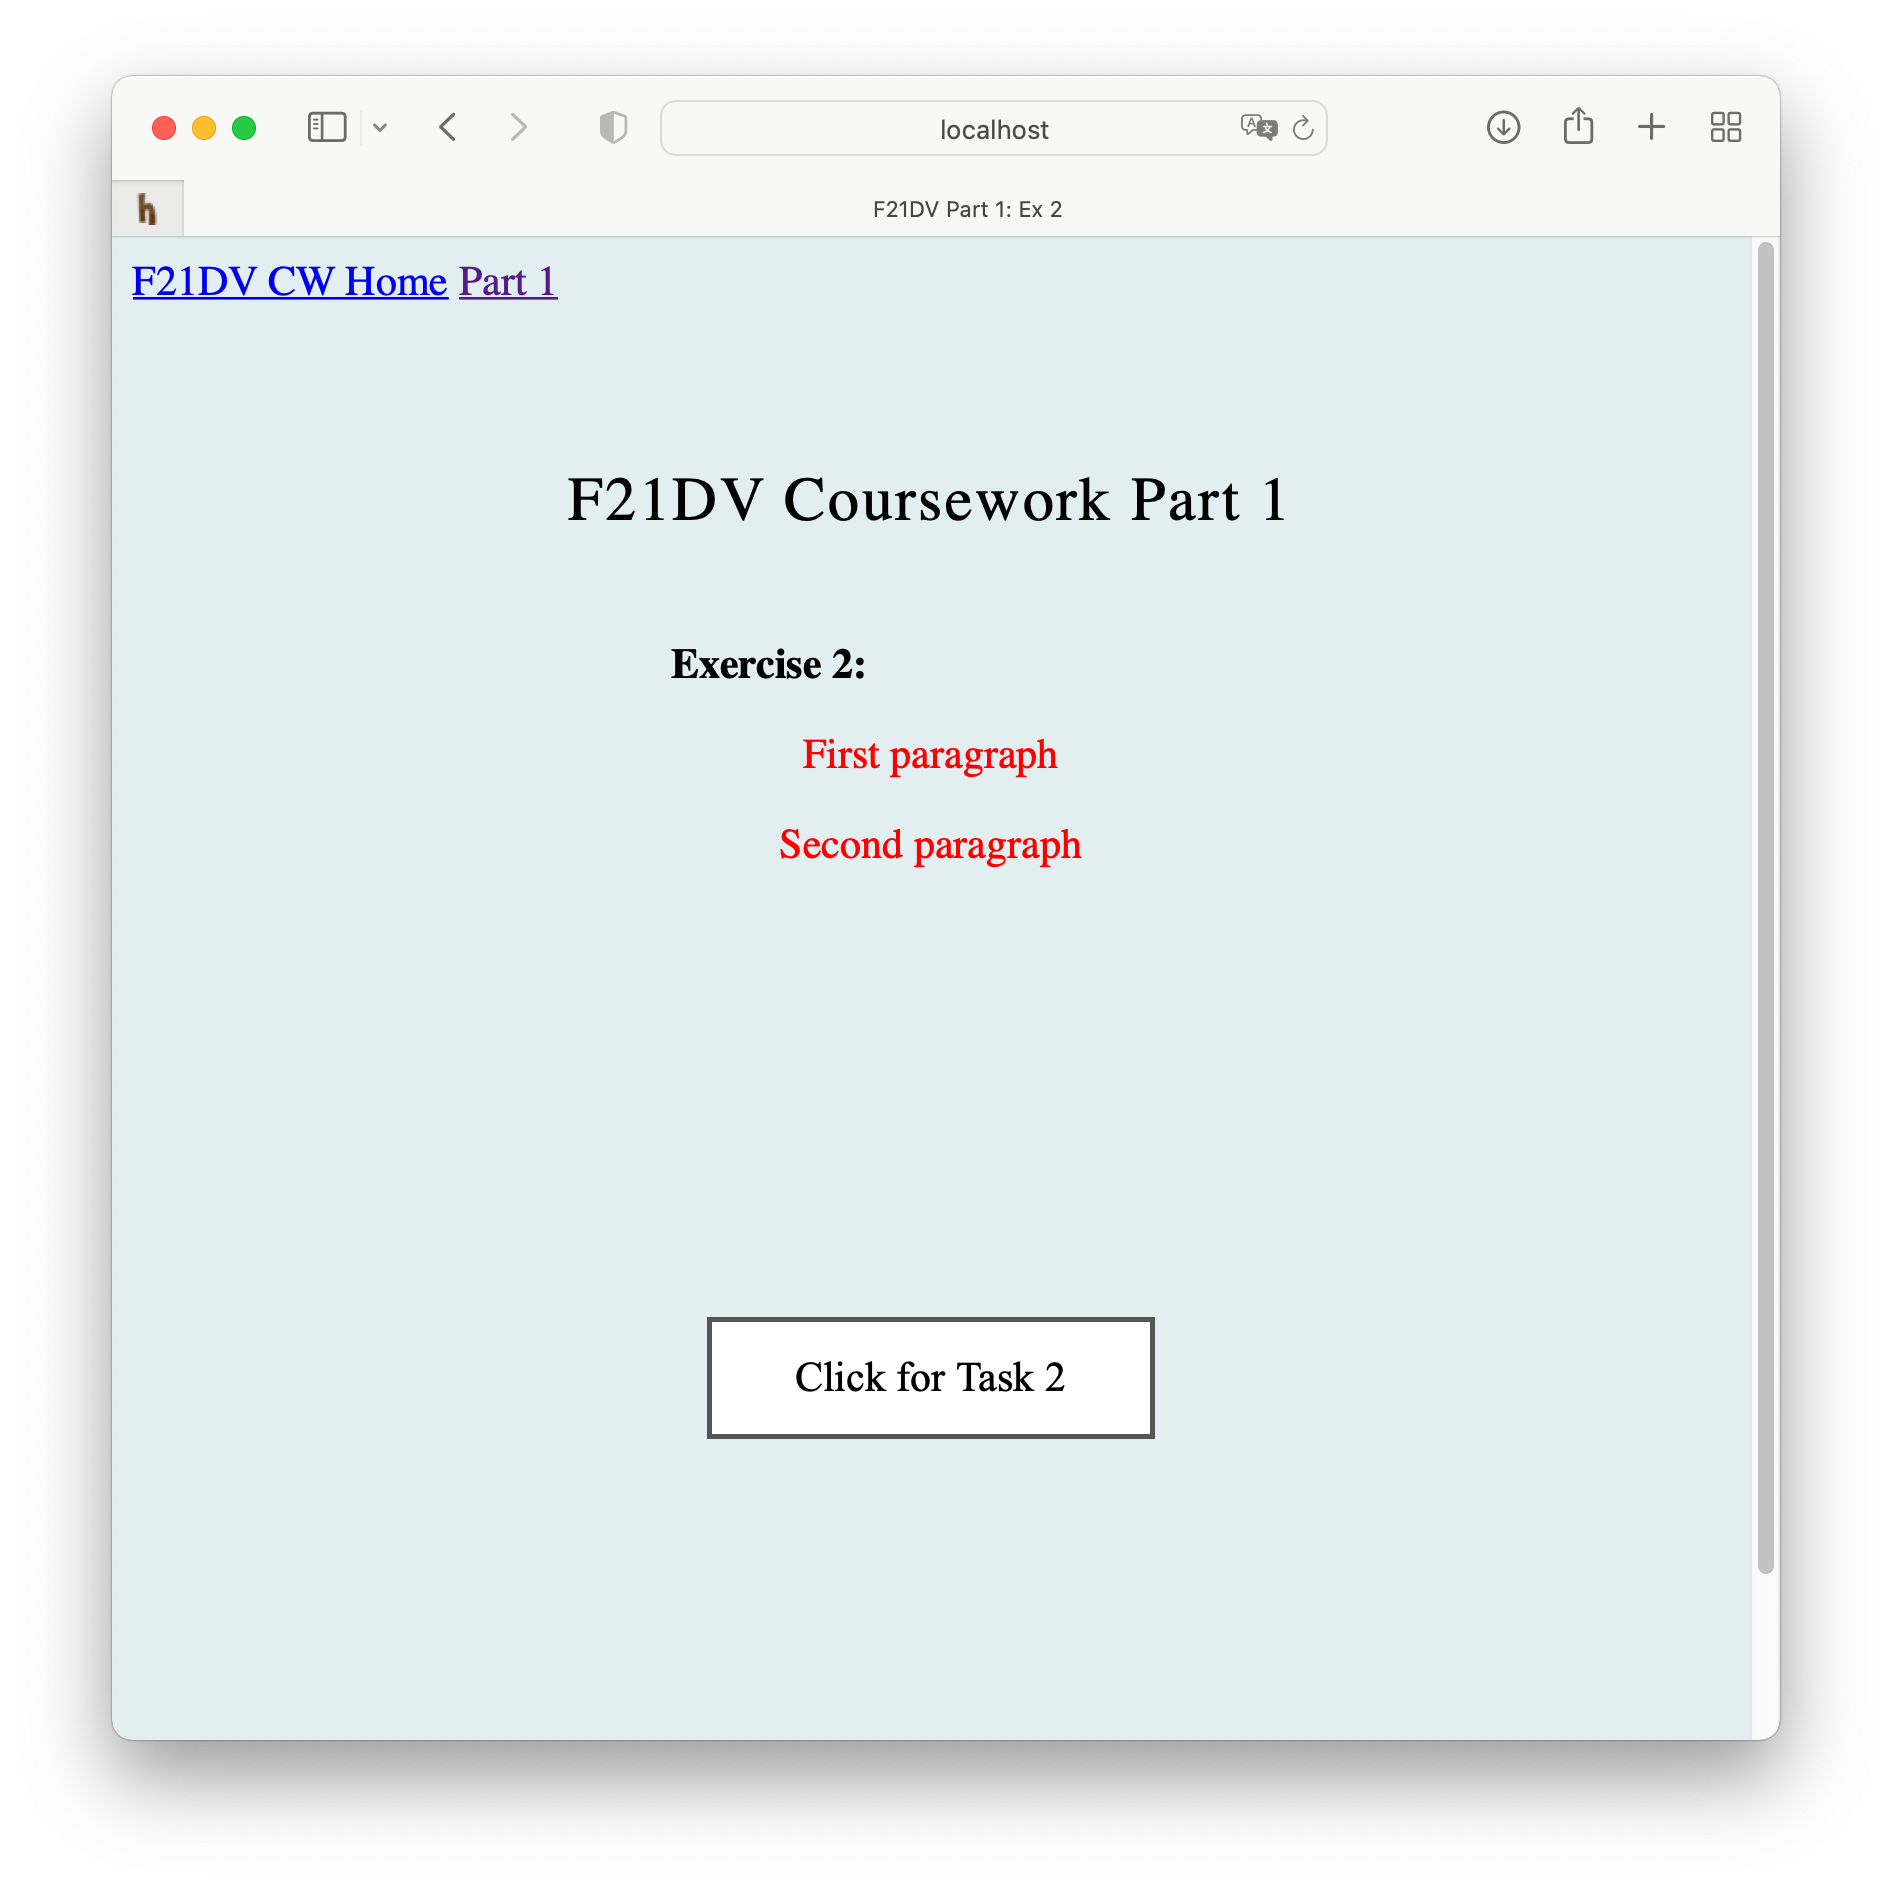
\includegraphics[width = 8cm]{images/ex2_2.png}
    \label{fig:ex2}
    \caption{Exercise 2}
\end{figure}
\FloatBarrier
Figure \ref{fig:ex2} shows that upon clicking the button, d3 would change the colours of the selected
\verb|<p>|s to red. 

\newpage
\section{Exercise 3 \& 4}
Exercises 3 \& 4 are one of the exercises where I have combined into one.
\begin{figure}[!ht]
    \centering
    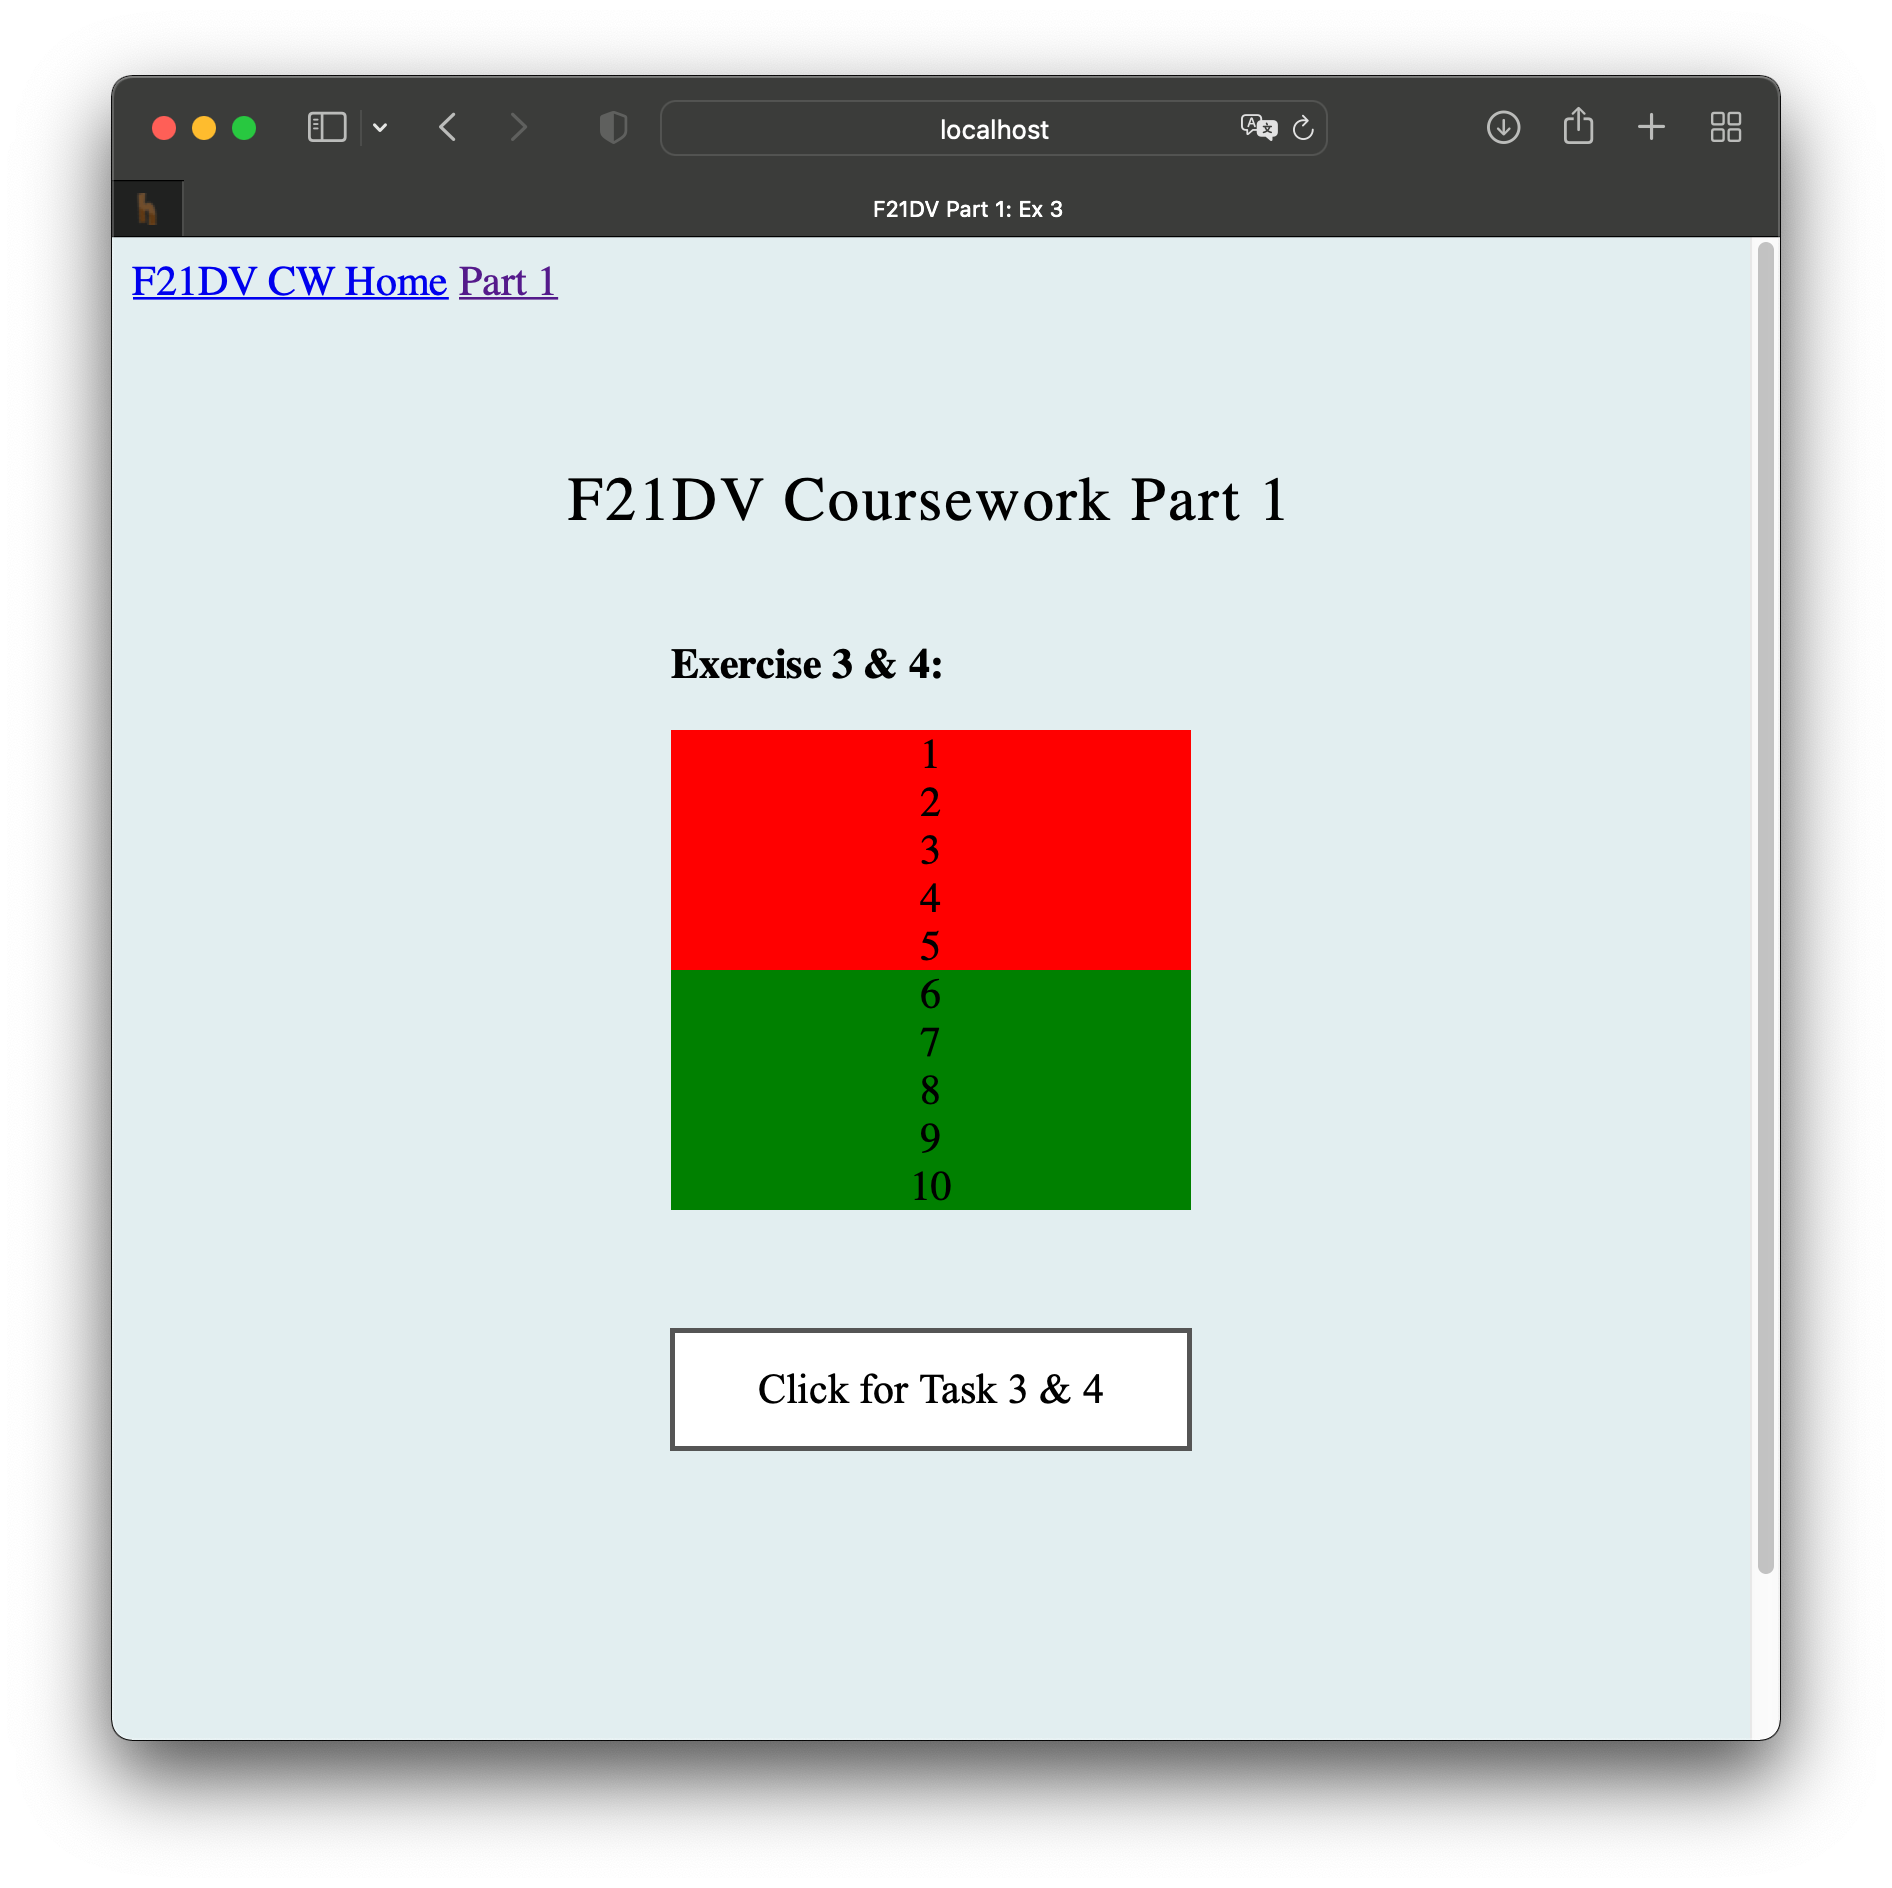
\includegraphics[width = 8cm]{images/ex3_1.png}
    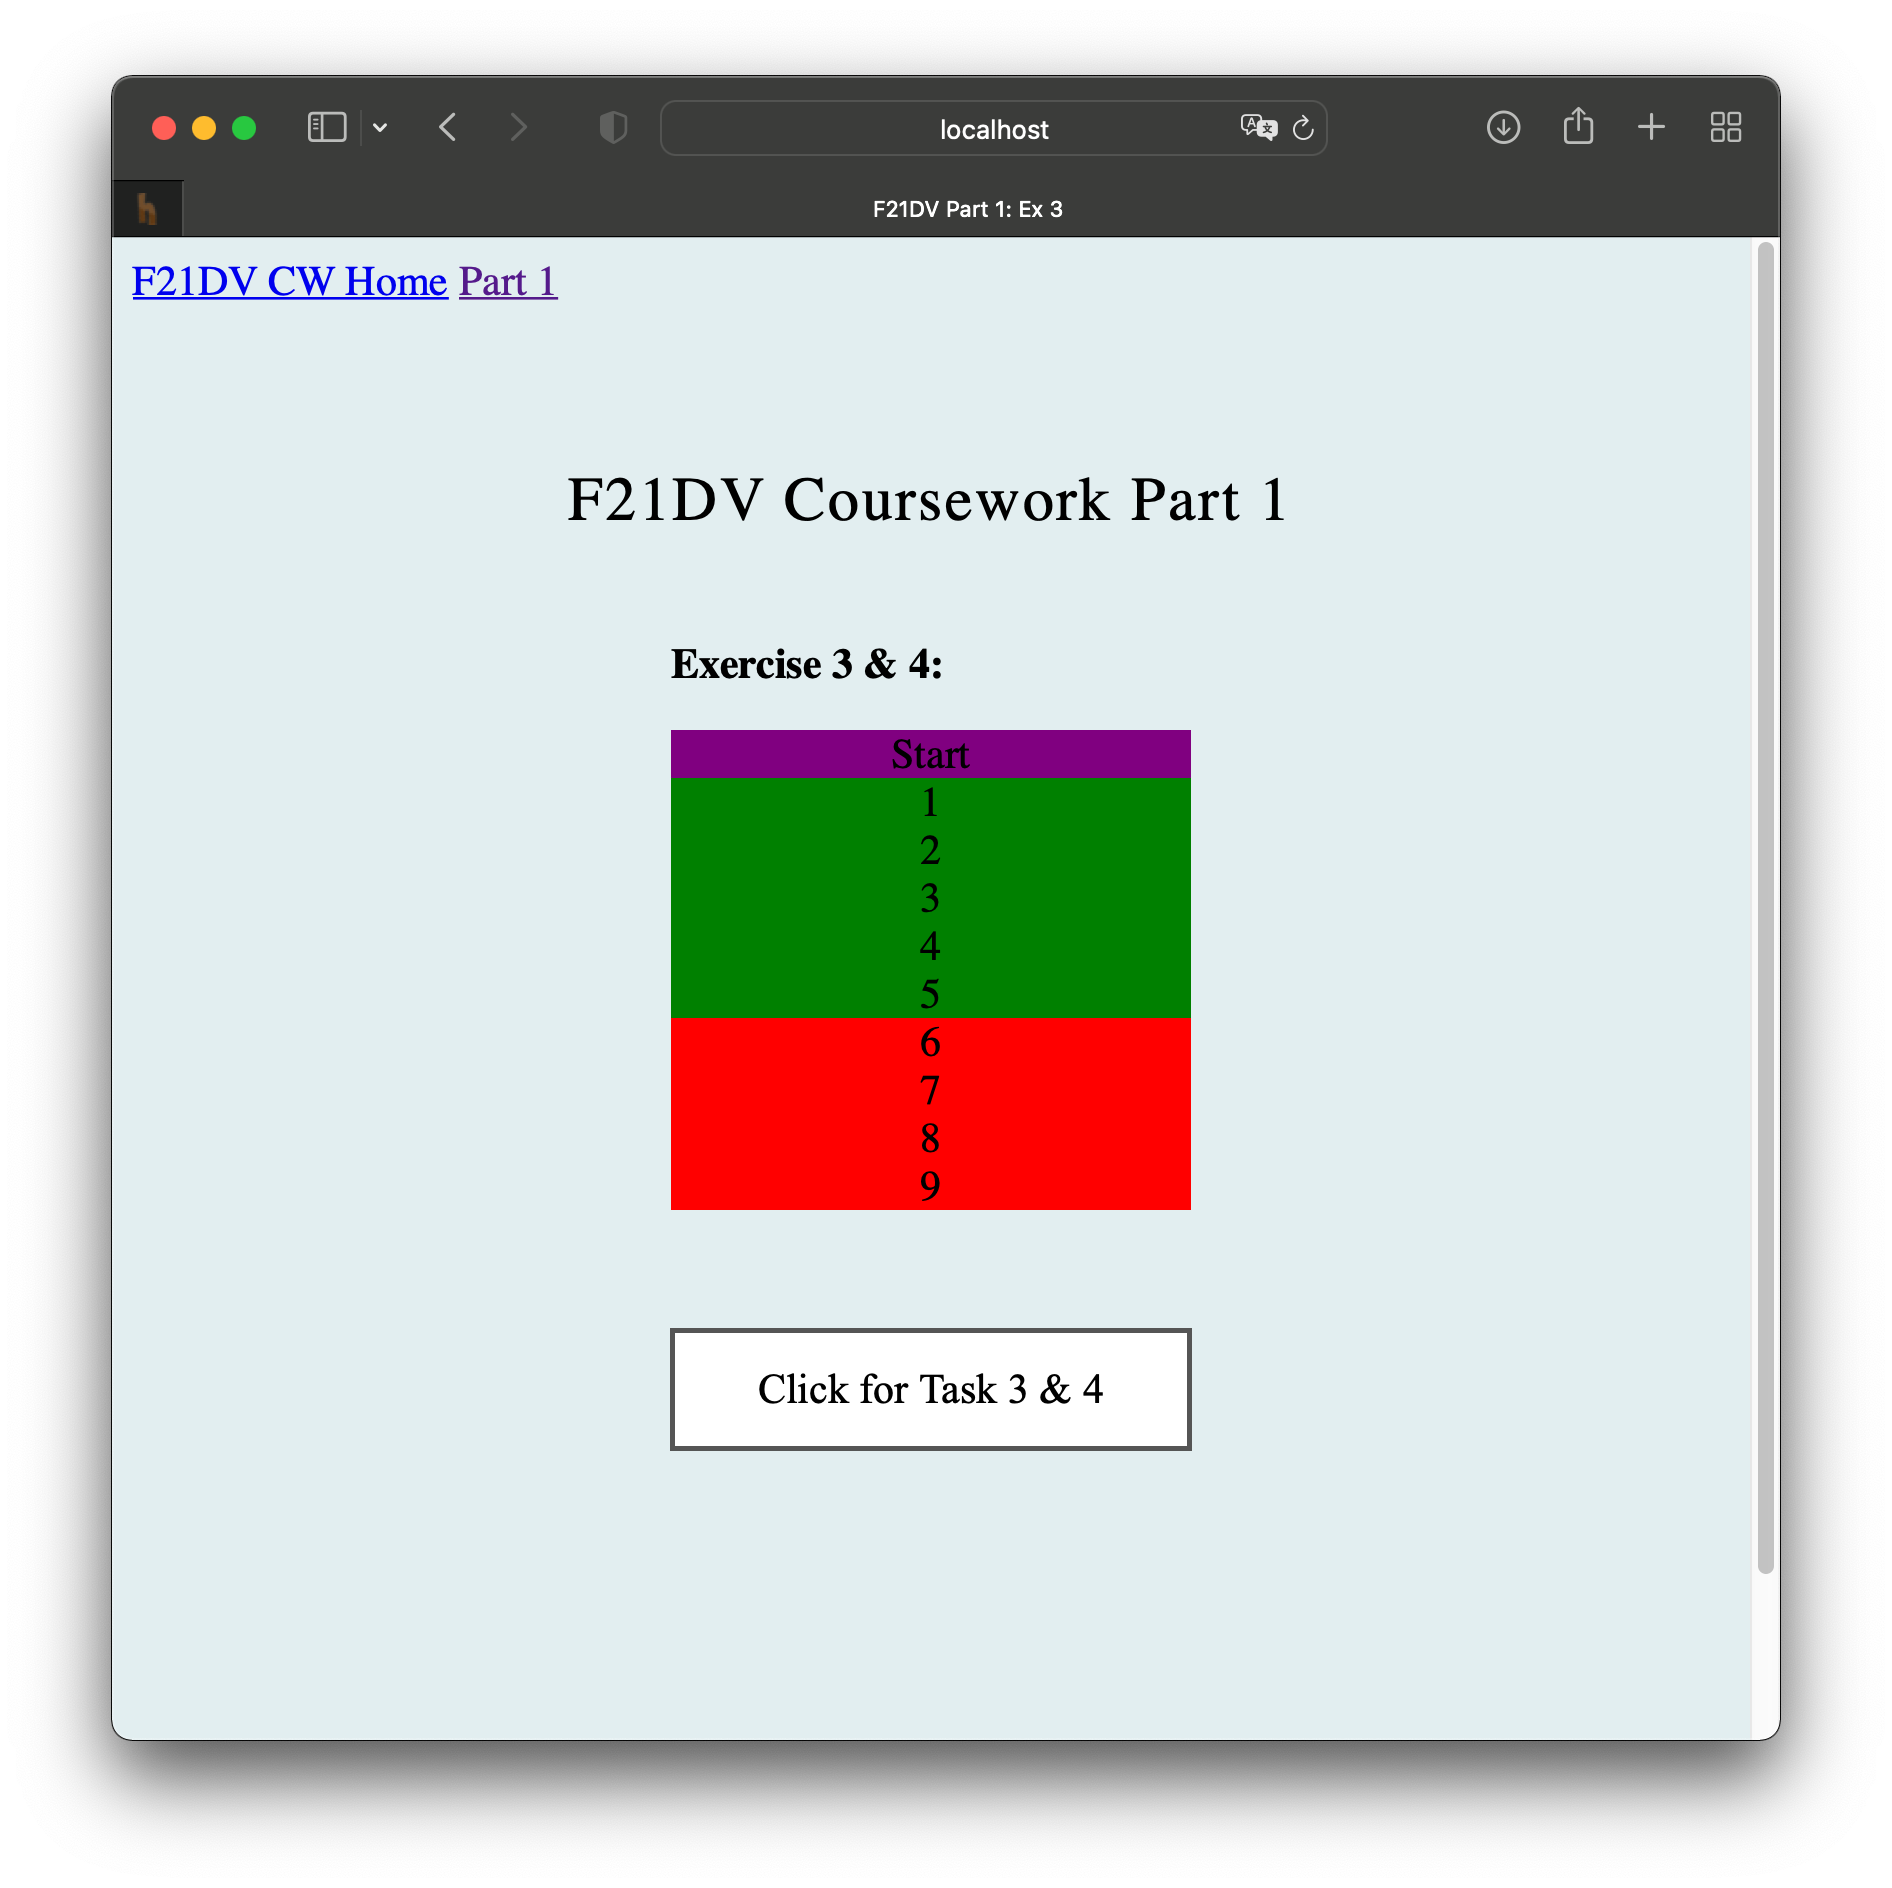
\includegraphics[width = 8cm]{images/ex3_2.png}
    \label{fig:ex3}
    \caption{Exercise 3}
\end{figure}
\FloatBarrier
Exercise 3 was to populate 10 div elements with numbers from 1 to 10, and to colour them according to
their values. Task four asks then, to replace the first value, "1", with the text "start". However, I
went ahead and implemented the change for the remaining divs as well, changing their values so that
the divs would show start, 1, 2, ..., 9, whilst keeping the colour requirements. Upon clicking the
button, the state of the div's would return to the original state again. Button is clickable multiple times.

\end{document}
